\input templates/header
%\documentclass{beamer}
% \usetheme[secheader]{Boadilla}
% \usecolortheme{beaver}
% \usefonttheme{serif}
% \usepackage{pgfpages}
% %\setbeameroption{show notes on second screen=right}
% 
% \AtBeginSection[]{
% \begin{frame}<beamer>[shrink]
% \frametitle{Contents}
% \begin{multicols}{2}
% %\tableofcontents[currentsection, hideothersubsections]
% \tableofcontents[currentsection]
% \end{multicols}
% \end{frame}
% }
% 
% \setbeamertemplate{navigation symbols}{}
% 
% \usepackage[utf8]{inputenc}
% \usepackage{hyperref}
% \usepackage{alltt}
% \usepackage{color}
% \usepackage{amsmath,amsfonts,amssymb,amsthm}
% \usepackage[ruled,vlined,nofillcomment]{algorithm2e}
% \usepackage{xspace}
% \usepackage{ds}
% \usepackage[normalem]{ulem}
% \usepackage{filemod}
% \usepackage{bibentry}
% \usepackage{multicol}
\usepackage{comment}
\usepackage{listings}


\newcommand{\Mapper}{\textsf{Mapper}\xspace}
\newcommand{\Reducer}{\textsf{Reducer}\xspace}
\newcommand{\Key}{\textit{key}\xspace}
\newcommand{\Values}{\textit{values}\xspace}
\SetKwData{EmitIntermediate}{EmitIntermediate}
\SetKwData{Emit}{Emit}
\SetKw{New}{new}
\SetKwFor{PROCEDURE}{}{}{}

\institute[UniTN]{University of Trento, Italy}
\author{Sabeur Aridhi}
\date[10.11.2014]{November 10, 2014}
\title[DS - Frameworks]{\textbf{Frameworks for Distributed Computing}}

\graphicspath{fig/12/}

\begin{document}

%-------------------------------------------------------------------------
\begin{frame}
\titlepage
\end{frame}

\begin{frame}
 \begin{center}
 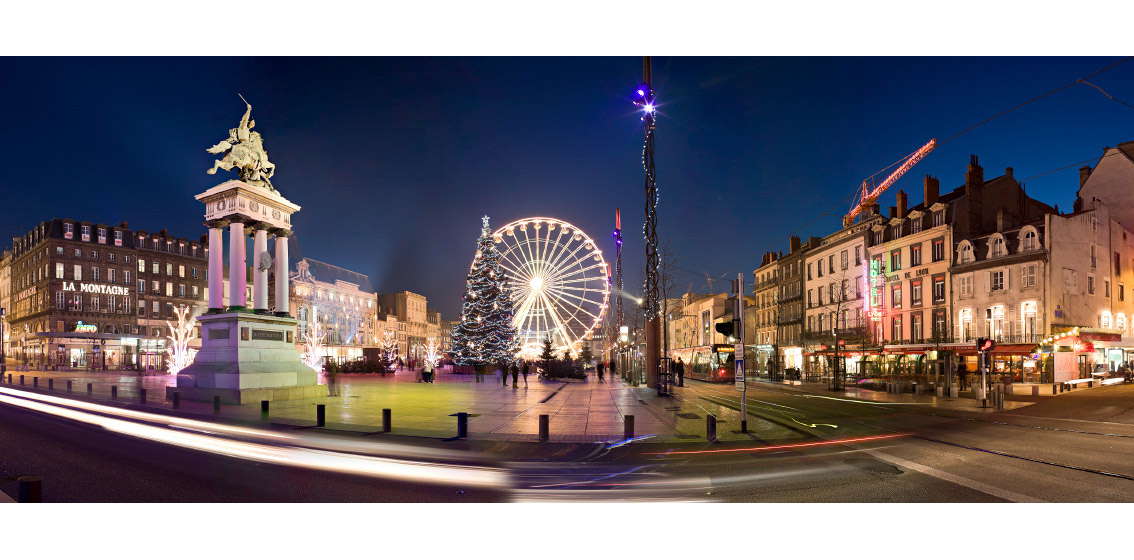
\includegraphics[keepaspectratio=true,width=\textwidth]{figs/12/clermont}
 \end{center}

\textbf{Sabeur Aridhi:} \\
 PhD at Blaise Pascal University, Clermont Ferrand, France.
\end{frame}

\section{Introduction}
\subsection{The problem}
% 
% \begin{frame}
%  \frametitle{So you are a young and fast growing company}
% \begin{center}
%  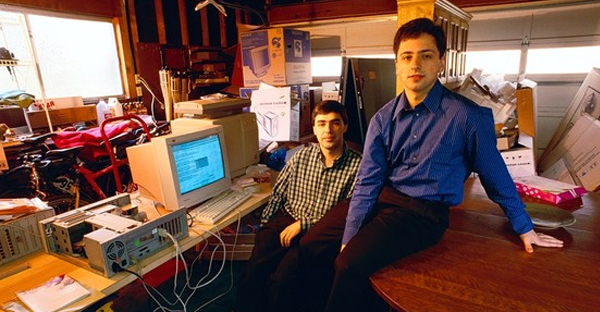
\includegraphics[keepaspectratio=true,scale=0.5]{figs/12/larry-page-sergey-brin-GOOGLE-early-days}
%  % 
%  % cpu.png: 871x868 pixel, 150dpi, 14.75x14.70 cm, bb=0 0 418 417
% \end{center}
% 
% \end{frame}
% 
% \begin{frame}
% \frametitle{Can your StartUp afford this?}
% \begin{columns} 
% \column{.4\textwidth} 
% \begin{center} 
%  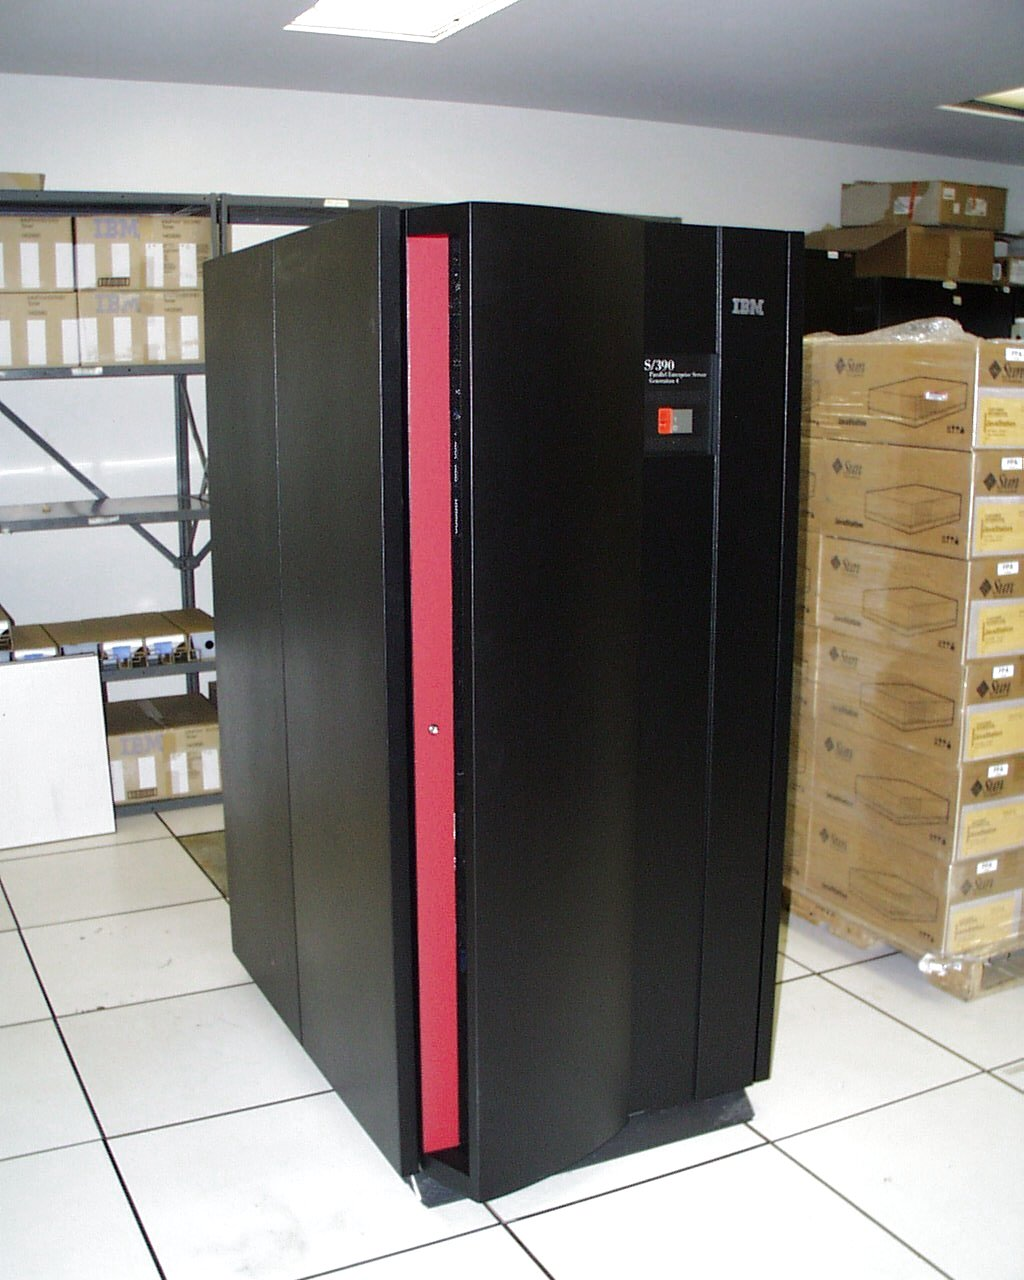
\includegraphics[keepaspectratio=true,scale=0.2]{figs/12/ibm_9672}
% \end{center} 
%  % http://www.yggdrasil.tv/galeria/view_photo.php?set_albumName=Procesadores
% \column{.6\textwidth} 
% IBM 9672, Prices available upon request. 
% \end{columns}
% \begin{block}{1 Unit, 5 years}<2->
% 6 958 684 Euro\footnote{\tiny in 2002: \url{http://www.fujitsu.com/downloads/ZA/whitepapers/openvme.pdf}}
% \end{block} 
% \end{frame}

\begin{frame}
 \frametitle{Growth of data size}
\begin{block}{Data sets}
 We need to analyze bigger and bigger datasets:
\begin{itemize}
 \item Web datasets: web topology (Google: est. 46 billion pages)
 % http://www.worldwidewebsize.com/
 \item Network datasets: routing efficiency analysis, tcp-ip logs
 \item Biological datasets: ontologies, genome sequencing data, protein folding patterns 
\end{itemize}

CPU speed of new computers is not growing fast enough.

Sequential algorithms are not a viable answer
\end{block}

\end{frame}

\begin{frame}
 \frametitle{Growth of CPU speed}
\begin{center}
	 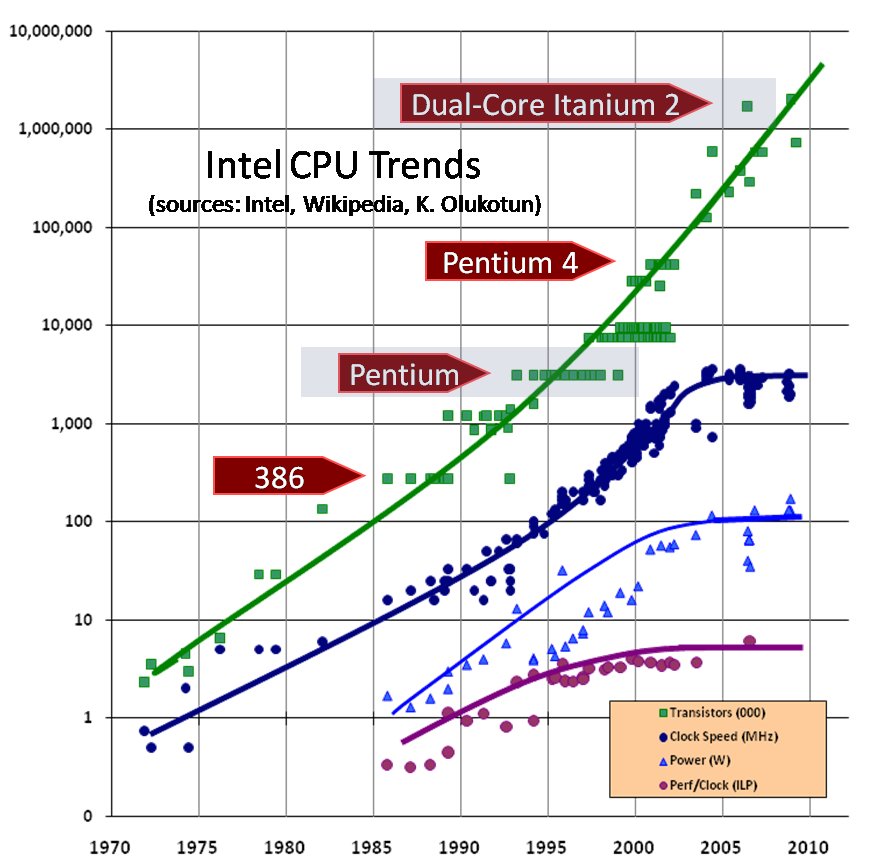
\includegraphics[keepaspectratio=true,scale=0.5]{figs/12/cpu.png}
 % cpu.png: 871x868 pixel, 150dpi, 14.75x14.70 cm, bb=0 0 418 417
\end{center}

\end{frame}

\subsection{Frameworks for distributed computing}

\begin{frame}
 \frametitle{Commodity Hardware to the Rescue}
\begin{block}{Approaches}
\begin{itemize}
\item Parallel algorithm
\item Distributed algorithms!
\end{itemize}
\end{block}


\begin{columns} 
\column{.48\textwidth} 
\begin{block}{Pros}
\begin{itemize}
 \item Cheaper
 \item Scalable
 \item More reliable
\end{itemize}
\end{block}

\column{.49\textwidth} 
\begin{block}{Cons}
\begin{itemize}
  \item More difficult to write
  \item Needs algorithm research
  \item Cluster maintenance
\end{itemize} 
\end{block}
\end{columns}
\end{frame}
\begin{comment}
\begin{frame}\frametitle{Parallel computing}
\begin{block}{Parallel vs Distributed}
 A parallel algorithm can have:
\begin{itemize}
 \item A global clock
 \item Shared memory
\end{itemize}
\end{block}

Are there ``easy ways'' to write parallel computing programs?

\begin{block}{Hands-on approach}
 Manually fire up threads, distribute data, etc\ldots
\end{block}
% \pause
% \vspace{-15em}
% \begin{center}
% 
\includegraphics[scale=0.6,keepaspectratio=true]{figs/12/dogscience}
% \end{center}
\end{frame}

\begin{frame}[fragile]
\frametitle{Parallel computing: OpenMP}
Easy way to parallelize a sequential program in shared memory:
\begin{block}{}
\begin{lstlisting}[language=c]
 #pragma omp parallel for private(w) reduction(+:sum)
 for(i = 0; i < N; i++){
      w = i*i;
      sum = sum + w*a[i];
 }
\end{lstlisting}
 
\end{block}

\begin{itemize}
 \item Can be tested as a sequential program
 \item Easy to understand
 \item Can be applied ``mostly'' on for cycles.
\end{itemize}
\end{frame}
\end{comment}
\begin{frame}\frametitle{Frameworks for distributed algorithms}
  \begin{itemize}
   \item Define a \textbf{Programming Model} that is inherently parallelizable.
   \item Give an interface to the programmer to implement the algorithm
   \item Create a \textbf{framework} that runs the program and gives fault-tolerance and scalability out of the box
  \end{itemize}

\end{frame}



\begin{frame}\frametitle{Target}
  We want a {\bf programming model} that is:
\begin{itemize}
 \item Transparent: the algorithm designer should not think about ``processes'' and ``messages''
 \item General 
 \item Intuitive
\end{itemize}
 We want a {\bf framework} that guarantees:
\begin{itemize}
 \item Failure resistance
 \item Scalability
 \item Locality
\end{itemize}
\end{frame}
% 
% \begin{frame}\frametitle{Scalability is not just a word:}
% \begin{center}
%  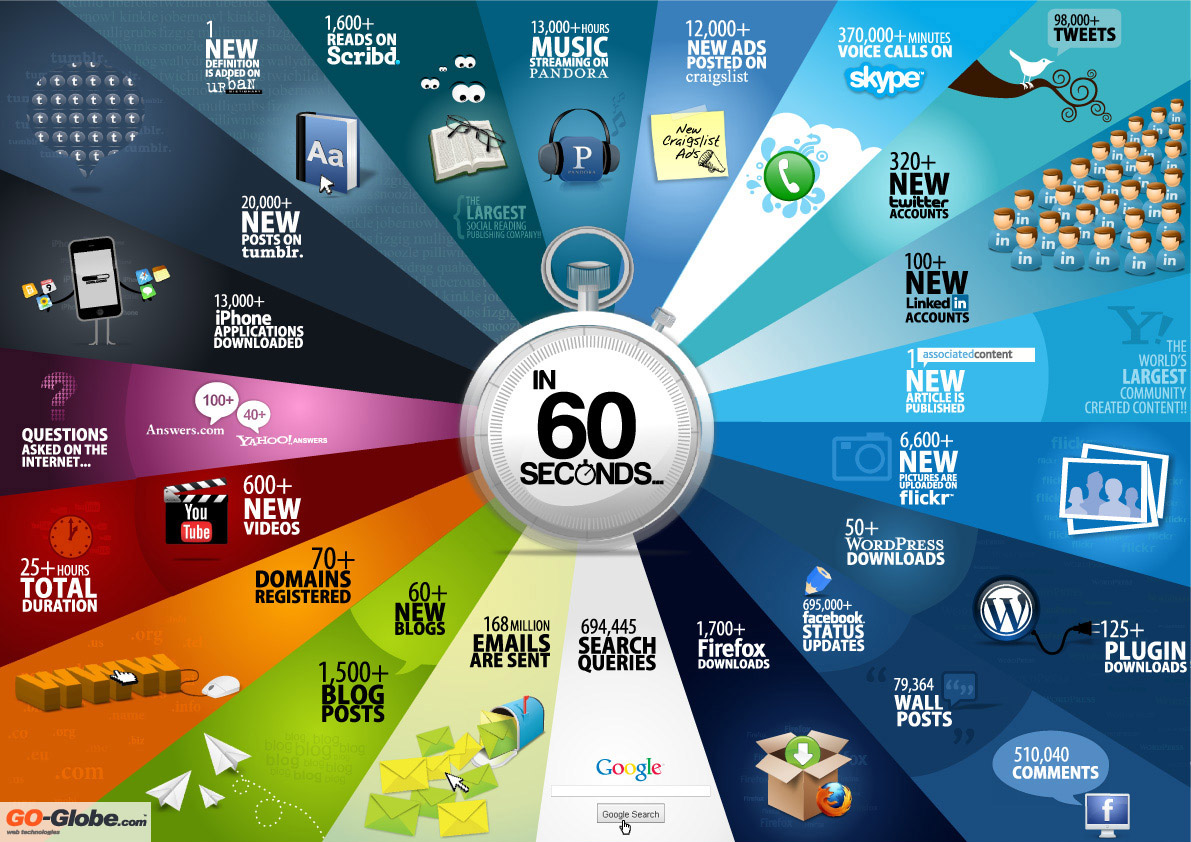
\includegraphics[keepaspectratio=true,scale=0.23]{figs/12/Infographic-60seconds-Large}
% 
%  \pause
%  Does one minute fit into RAM? Five Minutes?
% %https://digitalbuzz.s3.amazonaws.com/wp-content/uploads/2011/06/Infographic-60seconds-Large.jpg
%  \end{center}
% \end{frame}

\subsection{Assumptions}

\begin{frame}
 \frametitle{Distributed File System}
 Each of your computing nodes needs to access the data.
 %We assume the existance of a Distributed File System across our network.
 \vspace{2em}

 \begin{block}{Google's DFS}
 \begin{itemize}
  \item Data is replicated across the network. (Failure resistent, faster read operations).
  \item<2-> A ``namenode'' stores file metadata e.g. name, location of chunks
  \item<3-> A ``datanode'' stores chunks of that file
  \item<4-> A ``coherence'' of data and computation location is desirable
 \end{itemize}
 \end{block}
% Caveat:
%\begin{itemize}
% \item We want to ensure \textbf{locality}
% \item If the DFS and the Framework do not collaborate locality is unattainable
%\end{itemize}
\end{frame}

\begin{frame}
  \frametitle{Scenarios}
\begin{block}{Big companies}
Google, Yahoo, Microsoft have huge clusters of machines and huge data sets to analyze

A framework helps the developers use the cluster without expertise in distributed computing
\end{block}

% \begin{block}{Cloud computing}
%  The framework can be offered as a service by a provider e.g. Amazon EC2
% \end{block}
\end{frame}


\begin{frame}
  \frametitle{Scenarios}

\begin{block}{Cloud computing}
\begin{itemize}
\item Large number of computers that are connected via Internet.
\item Applications delivered as services.
\item Hardware and system software delivered as services.
\item Pay as you go.
\item Cloud services can be rapidly and elastically provisioned.

\end{itemize}
\end{block}
\begin{block}{Cloud computing}
 The framework can be offered as a service by a provider e.g. Amazon EC2
\end{block}
\end{frame}

\frame{\frametitle{Scenarios}
\begin{columns}
\begin{column}{0.6\textwidth}
  \includegraphics[width=180px, height=180px]{figs/12/cloudlayers.eps}
\end{column}

\begin{column}{0.4\textwidth}
\begin{block}{Service models}
\begin{itemize}
\item Software as a Service (SaaS).
\item Platform as a Service (PaaS),
\item Infrastructure as a Service (IaaS),
\end{itemize}
\end{block}
\end{column}
\end{columns}
}


\section{MapReduce}
\begin{frame}
\frametitle{History}

\begin{block}{Google, 2004:}
\begin{quotation}
MapReduce is a programming model and an associated
implementation for processing and generating large
data sets.
\end{quotation}
\end{block}

\begin{itemize}
\item Inspired by functional programming
\item Created to help Google developers to analyze huge datasets
\end{itemize}

\end{frame}

\subsection{Programming model}
% \begin{frame}
% \frametitle{Map and Reduce in functional programming}
% \begin{block}{Map function}
% Map: $(\alpha list, \alpha \rightarrow \beta) \rightarrow \beta list$ 
% \end{block}
% Example:
% Map([1,2,3], sqr)= [1,4,9]
% 
% \begin{block}{Reduce (or fold) function}
% Reduce: $(\alpha list, \beta, (\beta,\alpha) \rightarrow \beta) \rightarrow \beta$
% \end{block}
% Example:
% Reduce([1,2,3],0,+) = 6
% 
% \begin{block}{Compute Sum of squares of a list $l$:}
% Reduce(Map($l$,sqr),0,+)
% \end{block}
% 
% \end{frame}

\begin{frame}
\frametitle{Map and Reduce in MapReduce}
The user (you) must define two functions:

\begin{block}{Mapper}
Mapper: $(k_1,v_1) \rightarrow \text{list}(k_2,v_2)$
\end{block}

\begin{block}{Reducer}
Reducer: $(k_2,\text{list}(v_2)) \rightarrow \text{list}(v_3)$
\end{block}

\begin{itemize}
\item The Mapper function is executed concurrently.
\item $k_2, v_2$ are \textit{intermediate} pairs. 
\item Mapper results are grouped using $k_2$.
\item The Reducer function is executed concurrently.
\end{itemize}
\end{frame}

\begin{comment}
\begin{frame}
\frametitle{Map and Reduce in pictures}
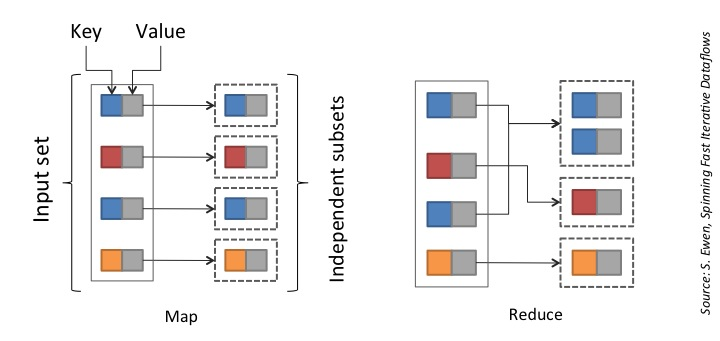
\includegraphics[width=\textwidth,keepaspectratio=true]{figs/12/SlidesFreytag/Slide11}
\end{frame}
\end{comment}

\begin{frame}
\frametitle{MapReduce flow (simplified)}
\begin{center}
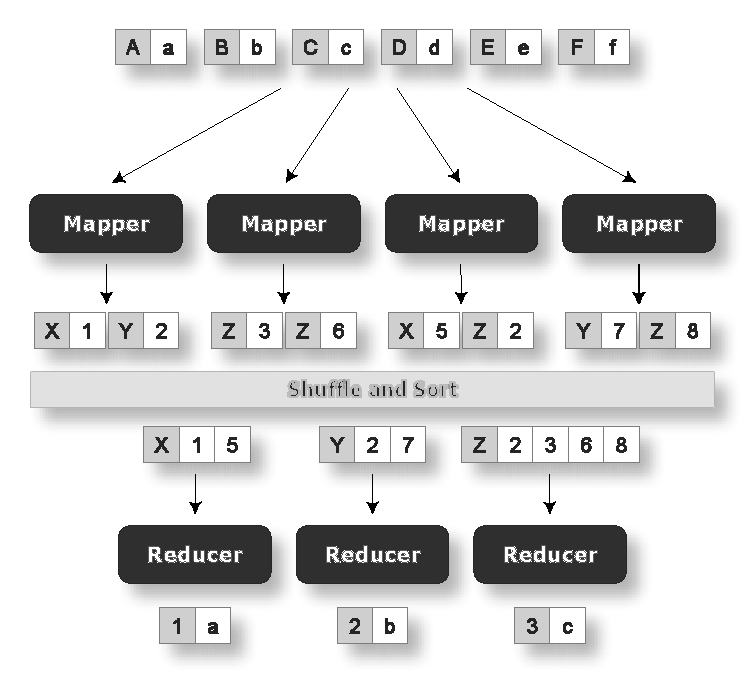
\includegraphics[scale=0.6,keepaspectratio=true]{figs/12/mapreduce_flow.pdf}
\end{center}

\end{frame}

\begin{frame}
\frametitle{Actually it is this way:}
\begin{itemize}
\item {\it Input is read from fs}
\item The Mapper function is executed concurrently.
\item {\it These results are written to fs}
\item {\it Input is read from fs}
\item The Reducer function is executed concurrently.
\item {\it These results are written to fs}
\end{itemize}
\end{frame}

\begin{frame}
\frametitle{Example: Word Count (MapReduce's Hello World)}
  \begin{block}{Input}
  A set of documents in a DFS
  \end{block}
  \begin{block}{Output}
  The number of occurrences of each word in the set of documents.
  \end{block}

  \begin{block}{Idea}<2->
  Work on each document concurrently and then ``reduce'' the results for each word.
  \end{block}

\end{frame}


\begin{frame}[fragile]
\frametitle{Example: Word Count (MapReduce's Hello World)}

\begin{algorithm}[H]
\KwIn{String filename, String content}
\SetKwFunction{Emit}{EmitIntermediate}
\SetKw{In}{in}
\ForEach{word w \In content}{
    \Emit{w,1}\;
}
\caption{Mapper}
\end{algorithm}

\vspace{-1em}
\begin{algorithm}[H]
\KwIn{String key, Iterator values}
\SetKwFunction{Emit}{Emit}
\SetKw{In}{in}
\SetKwData{Result}{result}
$\Result \leftarrow 0$\;
\ForEach{v \In values}{
    $\Result \leftarrow \Result + v$\;
}
\Emit(key,\Result)\;
\caption{Reducer}
\end{algorithm}
\end{frame}

\begin{frame} 
\frametitle{Possible optimization}
\begin{itemize}
  \item Creating a pair for each occurrence of each word looks like a waste of time
\end{itemize}

\begin{algorithm}[H]
\KwIn{String filename, String content}
\SetKwFunction{Emit}{EmitIntermediate}
\SetKw{In}{in}
\SetKw{New}{new}
$H \leftarrow \New$ HashTable\;
\ForEach{word w \In content}{
    $H[w]\leftarrow H[w] + 1$
}
\ForEach{word w \In H}{
    \Emit{w,$H[w]$}
}

\caption{Optimized-mapper}
\end{algorithm}
\end{frame}

\begin{frame}
\frametitle{Combiner and Partitioner}
\begin{block}{Combiner}

\begin{itemize}
  \item Insert a function between Mapper and Reducer.
  \item $Combiner: (k_2,\text{list}(v_2)) \rightarrow (k_2,\text{list}(v_3))$ 
  \item The combiner is applied before the global sort.
  \item Just like in the WordCount example.
\end{itemize}
\end{block}

\begin{block}{Partitioner}
  Before the global sort, control which reducer receives which key.
\end{block}
\end{frame}


\begin{frame}
\frametitle{Complete MapReduce flow}
\begin{center}
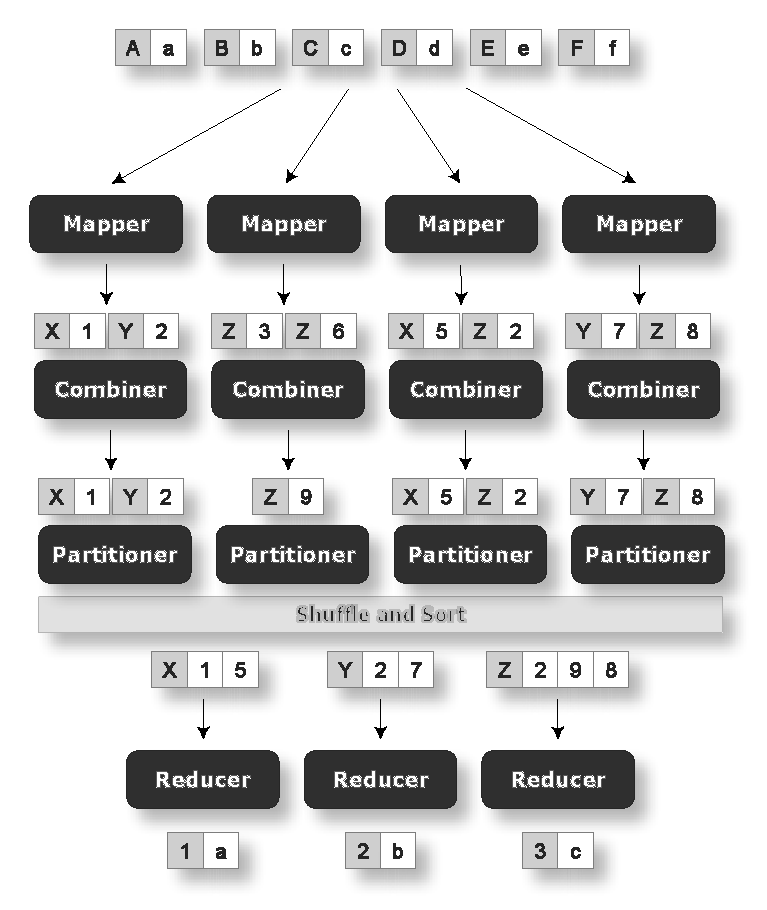
\includegraphics[scale=0.5,keepaspectratio=true]{figs/12/mapreduce_flow_full.pdf}
% mapreduce_flow.pdf: 363x329 pixel, 72dpi, 12.81x11.61 cm, bb=0 0 363 329
\end{center}

\end{frame}

\begin{frame}
\frametitle{Fault tolerance management}
% \begin{center}
% 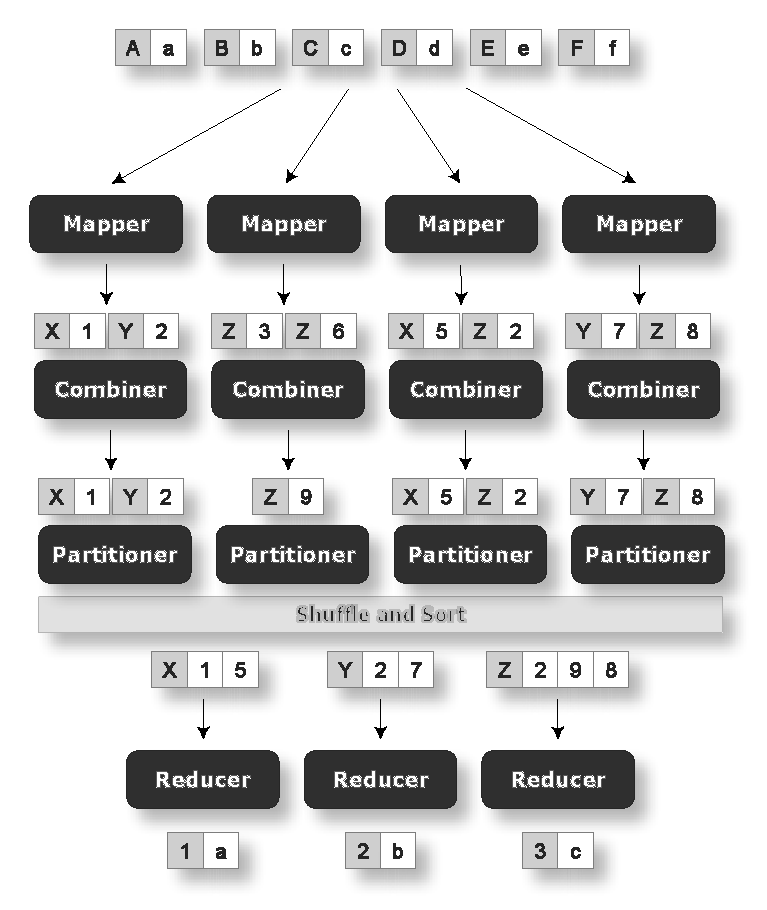
\includegraphics[scale=0.5,keepaspectratio=true]{figs/12/mapreduce_flow_full.pdf}
% mapreduce_flow.pdf: 363x329 pixel, 72dpi, 12.81x11.61 cm, bb=0 0 363 329
% \end{center}
\begin{itemize}
  \item Worker failure
      \begin{itemize}
      \item map (and not reduce) tasks completed reset to idle state
      \item map and reduce tasks in progress reset to idle
      \item Notification to and re-execution by workers executing reduce tasks
      \end{itemize}

  \item Master failure
  \begin{itemize}
      \item Version of 2004: 
      \begin{itemize}
      \item Abort the computation and retry
      \end{itemize}
      \item Other solution: 
      \begin{itemize}
      \item Periodic check points of the data structures 
      \item Launching of a new copy from the check point 
      \end{itemize}
      \end{itemize}
\end{itemize}
  



\end{frame}

\subsection{Framework}

\begin{frame}
\frametitle{Framework}

\begin{columns}
 \column{0.75\textwidth}
\begin{itemize}
\item Google's framework is not available
\item Open source alternative: Apache's Hadoop
\item Offered as service in Amazon Elastic Computing
\end{itemize}
 \column{0.2\textwidth}
 
\includegraphics[width=\textwidth,keepaspectratio=true]{figs/12/hadoop}
\end{columns}
\end{frame}

\begin{frame}
\frametitle{Overview}
\begin{center}
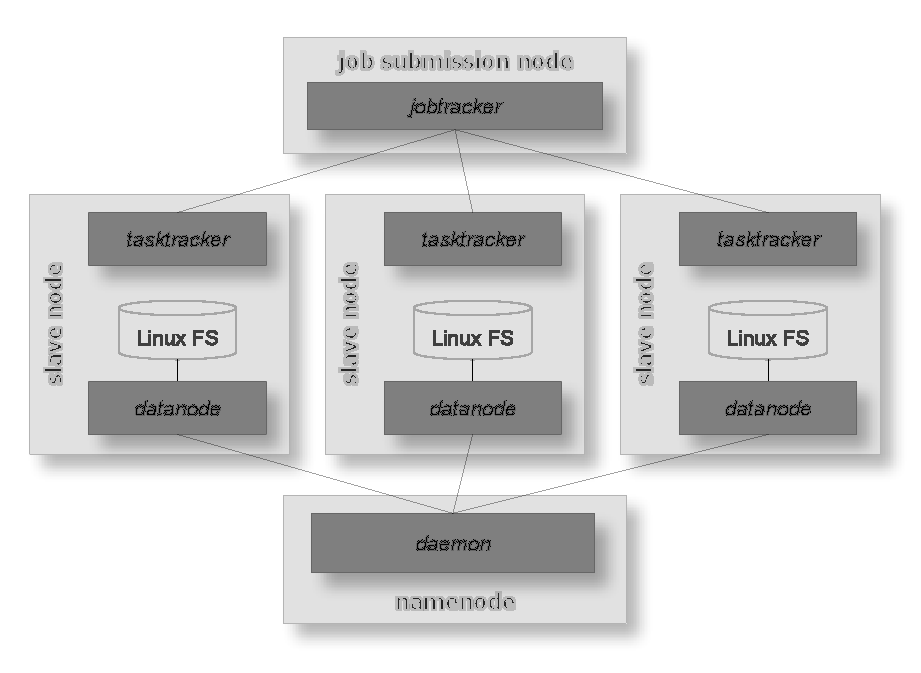
\includegraphics[scale=0.7,keepaspectratio=true]{figs/12/hadoop_arch.pdf}
% mapreduce_flow.pdf: 363x329 pixel, 72dpi, 12.81x11.61 cm, bb=0 0 363 329
\end{center}

\end{frame}


\begin{frame}
\frametitle{Hadoop Details}
\begin{itemize}
\item Library in Java
\item Started by Yahoo in 2006
\item Driver program must be written in Java
\item Possibility to use external programs as mapper and reducers
\item Relatively stable
% \item Current de-facto Standard
\end{itemize}
\end{frame}

\subsection{Algorithms}
\begin{frame}
%\frametitle{Inverted Index (Job interview question ;)}
\frametitle{Inverted Index (Job interview question ;)}
\begin{block}{Problem}
  We are given a set of webpages $P=\{P_1,\ldots,P_n\}$. 
  
  We want to know for each word in the dataset, in which documents it appears (and how many times)
\end{block}
\end{frame}

\begin{frame}
\frametitle{MapReduce flow (simplified)}
\begin{center}
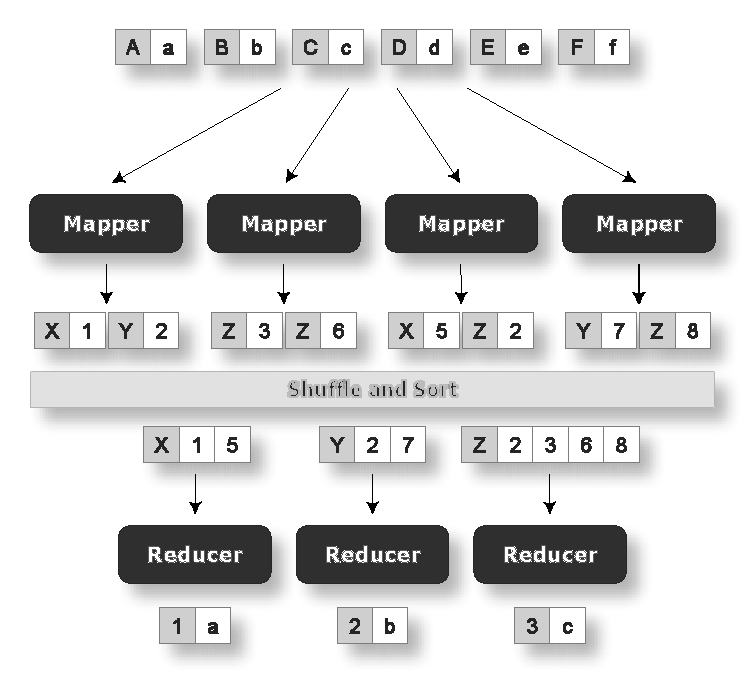
\includegraphics[scale=0.6,keepaspectratio=true]{figs/12/mapreduce_flow.pdf}
% mapreduce_flow.pdf: 363x329 pixel, 72dpi, 12.81x11.61 cm, bb=0 0 363 329
\end{center}
\end{frame}

\begin{frame}
\frametitle{Baseline solution}


\begin{algorithm}[H]
%\KwIn{String filename, String content}
\SetKwFunction{Emit}{EmitIntermediate}
\SetKw{In}{in}
\SetKw{New}{new}
$H \leftarrow \New$ HashTable\;
\ForEach{word w \In content}{
    $H[w]\leftarrow H[w] + 1$
}
\ForEach{word w \In H}{
    \Emit{w,$(filename,H[w])$}
}
\caption{Mapper(String filename, String content)}
\end{algorithm}

\vspace{-1em}
\begin{algorithm}[H]
%\KwIn{String key, Iterator values}
\SetKwFunction{Emit}{Emit}
\SetKw{In}{in}
\SetKwData{Result}{result}
$\Result \leftarrow []$\;
\ForEach{v \In values}{
    $\Result.add(v)$\;
}
$\Result.sortbyfreq()$\;
\Emit(key,\Result)\;
\caption{Reducer(String key, Iterator values)}
\end{algorithm}
\end{frame}

\begin{frame}
\frametitle{Simple run}
\begin{center}
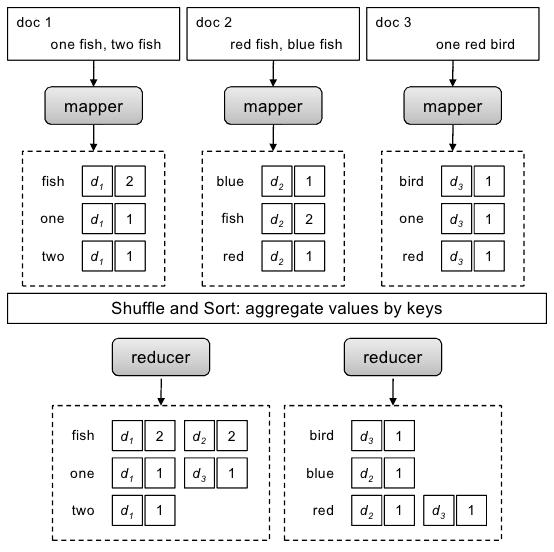
\includegraphics[scale=0.5,keepaspectratio=true]{figs/12/invindexing.jpeg}
% mapreduce_flow.pdf: 363x329 pixel, 72dpi, 12.81x11.61 cm, bb=0 0 363 329
\end{center}
\end{frame}

\begin{frame}
	\frametitle{K-Means clustering}
  \begin{block}{Problem definition}
  Given a set of points, partition them to minimize the within-cluster sum of squares
  \end{block}
	
\begin{block}{Standard algorithm (LLoyd 1982)}
      \begin{itemize}
	\item Choose K centroids at random
	\item While changes:
	  \begin{itemize}
	  \item Assign each point to closest centroid
	  \item Move each centroid to the average of the points assigned to it
	  \end{itemize}
      \end{itemize}
      \end{block}
\end{frame}

\begin{frame}
      \frametitle{K-Means run}
    \begin{center}
	  \only<1>{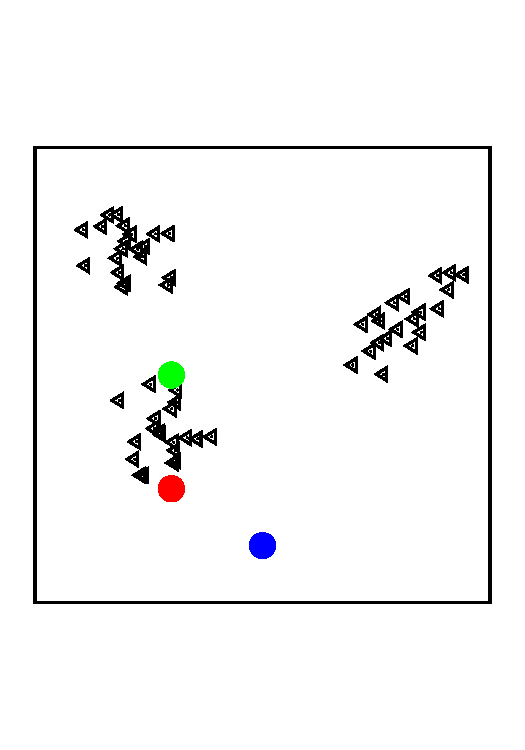
\includegraphics[angle=270,width=.8\textwidth]{figs/12/step1.pdf}}
      \only<2>{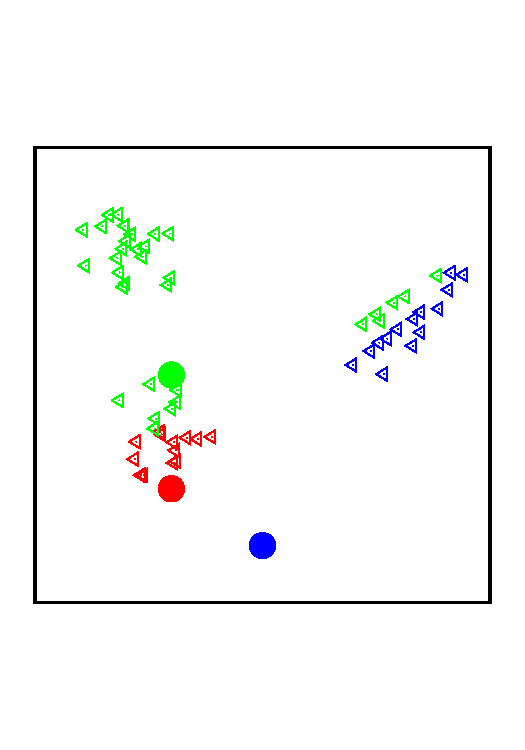
\includegraphics[angle=270,width=.8\textwidth]{figs/12/step2.pdf}}
      \only<3>{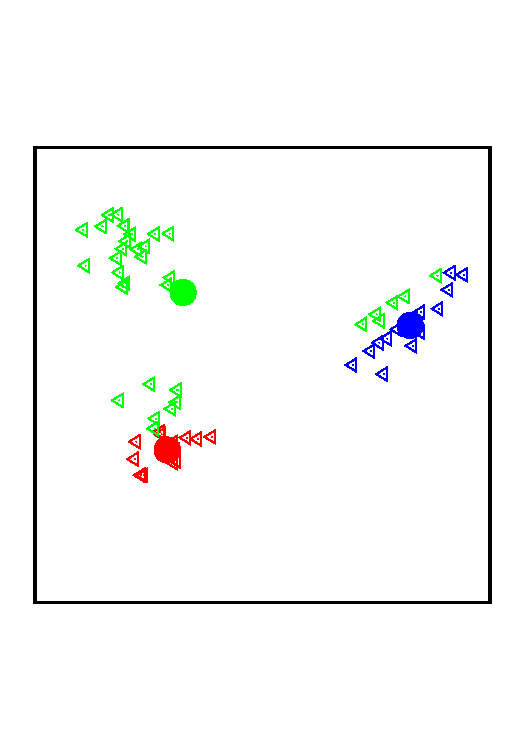
\includegraphics[angle=270,width=.8\textwidth]{figs/12/step3.pdf}}
      \only<4>{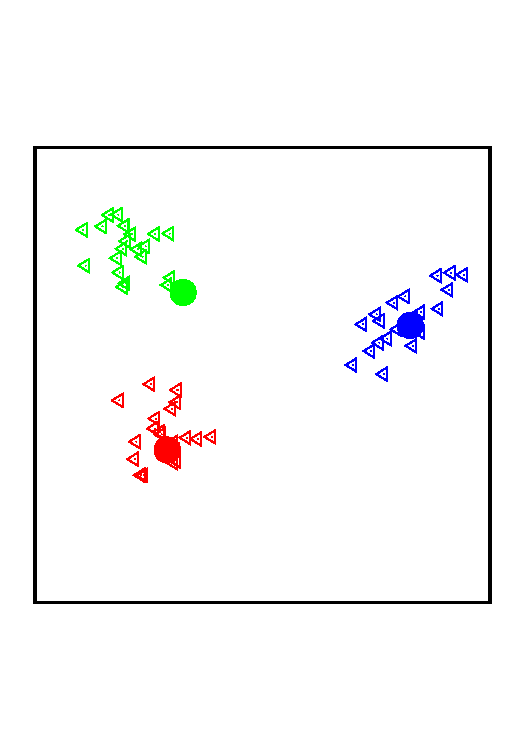
\includegraphics[angle=270,width=.8\textwidth]{figs/12/step4.pdf}}
      \only<5>{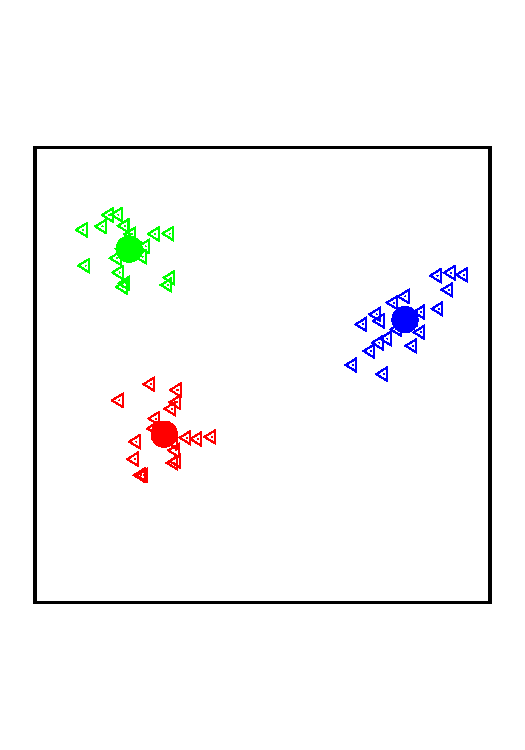
\includegraphics[angle=270,width=.8\textwidth]{figs/12/step5.pdf}}
    \end{center}
\end{frame}

\begin{frame}
\frametitle{MapReduce Algorithm}
\begin{itemize}
\item Impossible to solve in a single job
\item Each MapReduce job corresponds to a KMeans step
\item We need a ``driver'' program.
\end{itemize}
\begin{block}{Driver}
\begin{itemize}
  \item Let $C'$ be the set of starting centroids
  \item Do: 
  \begin{itemize}
      \item Set $C = C'$
      \item Send $C$ to all nodes
      \item Run MapReduce algorithm
      \item Extract new centroids $C'$ from output 
  \end{itemize}
  \item While $C \neq C'$
\end{itemize}
\end{block}
\end{frame}

\begin{frame}
\frametitle{MapReduce Algorithm}

\begin{algorithm}[H]
\KwIn{Int id, Point p}
\SetKwFunction{Emit}{EmitIntermediate}
\SetKwData{K}{k}
\SetKw{In}{in}
\SetKw{Argmin}{argmin}
$\K \leftarrow \Argmin_i(dist(p,C_i))$ \;
\Emit{\K,p}\;
\caption{Mapper}
\end{algorithm}

\begin{algorithm}[H]
\KwIn{centroid$_{id}$, Iterator points}
\SetKwFunction{Emit}{Emit}
\SetKw{In}{in}
\SetKw{Avg}{avg}
\SetKwData{Result}{result}
$\Result \leftarrow \Avg(points)$\;
\Emit(centroid$_{id}$,\Result)\;
\caption{Reducer}
\end{algorithm}
\end{frame}

\subsection{Extensions}
\begin{frame}
 \frametitle{Extensions over Hadoop MapReduce}
 \begin{itemize}
  \item Give higher level abstraction
  \item No need to think in terms of maps and reduces
  \item Easier to use
 \end{itemize}
\end{frame}
\begin{comment}
\subsubsection{Sawzall}
\begin{frame}
 \frametitle{Sawzall}
 \begin{itemize}
  \item Developed by Google
  \item Used for simple queries
  \item Target: a distributed awk. 
 \end{itemize} 

\end{frame}

\begin{frame}[fragile]
 \frametitle{Example}
 \begin{block}{Problem}
  Given a dataset of real numbers, compute how many numbers there are, the sum and the sum of squares
 \end{block}

\begin{block}{Code}
 \begin{verbatim}
count: table sum of int;
total: table sum of float;
sum_of_squares: table sum of float;
x: float = input;
emit count <- 1;
emit total <- x;
emit sum_of_squares <- x * x; 
\end{verbatim}
\end{block}

\end{frame}

\begin{comment}
\begin{frame}[fragile]
 \frametitle{Other Aggregators}
 \begin{verbatim}
c: table collection of string;
s: table sample(100) of string;
m: table maximum(10) of string weight length: int;
q: table quantile(101) of response_in_ms: int;
t: table top(10) of language: string;
\end{verbatim}
 
\end{frame}
\end{comment}

\subsubsection{Hive}

\begin{frame}
 \frametitle{Hive}
\begin{columns}
 \column{0.75\textwidth}
 \begin{itemize}
  \item Developed and used at Yahoo.
  \item Database warehouse on top of Hadoop (Warehouse == offline, high latency)
  \item Goals: Easy data summarization, ad-hoc querying and analysis of large volumes of data. 
  \item SQL like syntax
  \item Extend Hive via custom MapReduce jobs
  \item Facebook uses it to scan 135 TB of compressed data / day (2010)
\end{itemize}
 \column{0.23\textwidth}
 
\includegraphics[width=\textwidth,keepaspectratio=true]{figs/12/hive_logo}
\end{columns}
\end{frame}

\begin{comment}

\subsubsection{Pig-Latin}

\begin{frame}
 \frametitle{Pig-Latin}
 \begin{itemize}
  \item Developed and used at Yahoo.
  \item ``designed to fit in a sweet spot between the declarative style
of SQL, and the low-level, procedural style of map-reduce.''
\end{itemize}
\end{frame}

\begin{frame}[fragile]
 \frametitle{Example}
 \begin{block}{SQL query}
\begin{verbatim}
SELECT category, AVG(pagerank)
FROM urls WHERE pagerank > 0.2
GROUP BY category HAVING COUNT(*) > 1000000  
\end{verbatim}
 \end{block}

\begin{block}{Pig-Latin program}
\begin{verbatim}
good_urls = FILTER urls BY pagerank > 0.2;
groups = GROUP good_urls BY category;
big_groups = FILTER groups BY COUNT(good_urls)>1000000;
output = FOREACH big_groups GENERATE
category, AVG(good_urls.pagerank);
\end{verbatim}

\end{block}
\end{frame}


\begin{frame}
 \frametitle{Notes}
\begin{center}
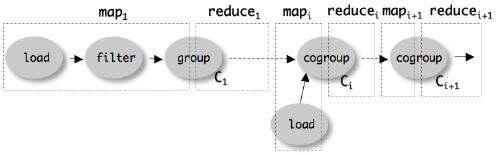
\includegraphics[width=\textwidth,keepaspectratio=true]{figs/12/piglatin.jpeg}
\end{center}
\begin{itemize}
 \item The program is decomposed in different MapReduce jobs
 \item Full support for User Defined Function
 \item Has a debugging tool
\end{itemize}
\end{frame}
\end{comment}

\begin{frame}{MapReduce: Use and abuse}

Hadoop horror stories (from Yahoo)
\begin{itemize}
\item Map tasks that take a full machine for 3 days
\item Jobs that have 10 MB of data per task, but 1 GB of data in distributed cache
\item Running MPI on Hadoop clusters by having a MapReduce job that launches MPI in reducers
\end{itemize}

\bigskip
What are the problems?
\begin{itemize}
\item Iterative data-flows are not optimized
\item The entire state must be input again at each iteration
\end{itemize}

\end{frame}

% \begin{frame}
%  \frametitle{Defects}
% \begin{itemize}
%  \item Each MapReduce cycle $\#nodes \times$ 2 write and 2 read operations.
%  \item Joining needs a whole MapReduce cycle, before any actual computation is done.
% \end{itemize}
% 
% \begin{block}{Recap: Join}<2->
% Dog(Dog, Name) $\Join$ Food(Kind, Name) = (Dog, Name, Kind)
% 
% \vspace{2pt}
% translates to:
% 
% \vspace{2pt}
% map([Dog, Name]) = Name, $\{$Dog, Dog$\}$\\
% map([Kind, Name]) = Name, $\{$Kind, Food$\}$\\ 
% reduce(Name, [$\{$Kind, Food$\}$, $\{$Dog, Name$\}$]) = $\{$Name, Kind, Food$\}$
% 
% \end{block}
% \pause
% \begin{center}
% \color{red}{2 Maps and huge data traffic!}
% \end{center}
% \end{frame}

\section{Other frameworks}
\begin{frame}
\frametitle{Why another framework?}
\begin{itemize}
\item MapReduce is merely a starting point, not a solution
\item Why Key/Value? Why not Key/Tuple?
\item Why only {\tt map()} and {\tt reduce()}
\item Can I reorder functions? Can I combine some?
\item Can a computer do this for me?
\end{itemize}
\end{frame}

% \begin{frame}
% \frametitle{Wait, reordering?}
% \begin{center}
% {Your database does this all the time!}
% 
% 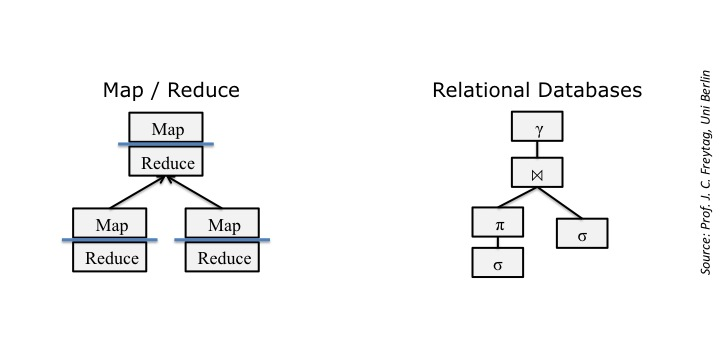
\includegraphics[width=0.9\textwidth,keepaspectratio=true]{figs/12/SlidesFreytag/Slide03}

% {However MapReduce does not define Semantics, or even Schema information}
% \end{center}
% \end{frame}

\subsection{SPARK}
\begin{frame}
\frametitle{Framework}
\begin{block}{SPARK framework}
\begin{itemize}
\item A general engine for large-scale data processing.
\item It combines SQL, streaming, and complex analytics.
\item It offers several high-level operators that make it easy to build parallel applications.
\end{itemize}

\end{block}

\centering
 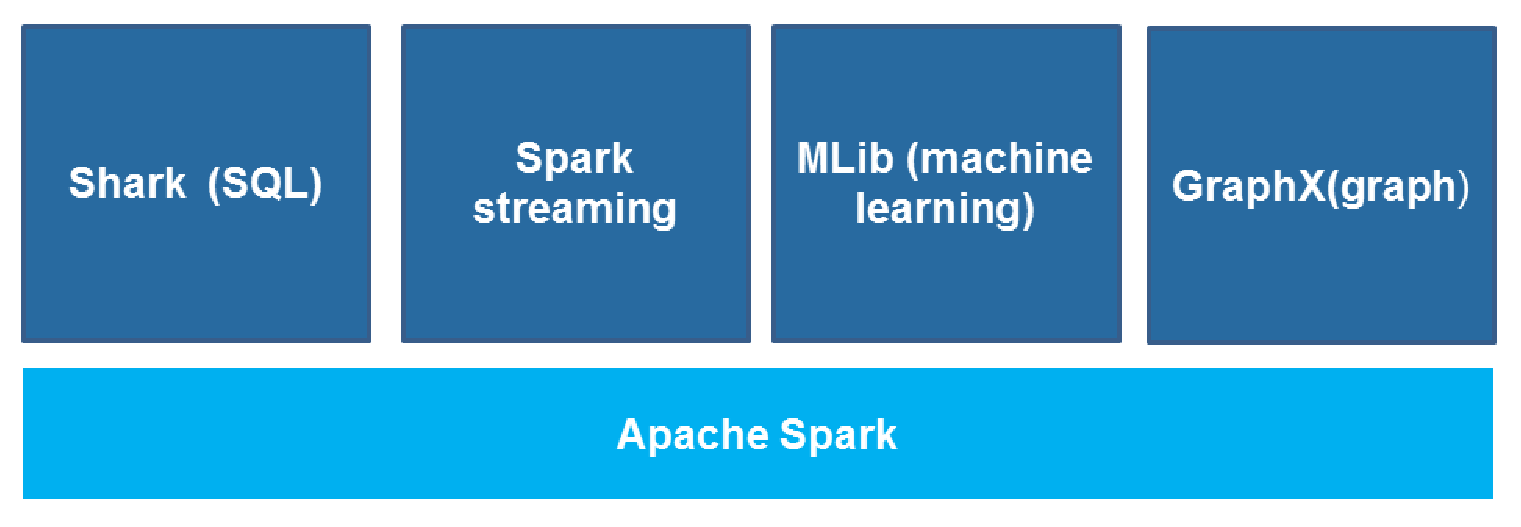
\includegraphics[width=220px, height=110px]{figs/12/spark.eps}
\end{frame}

\begin{frame}
\frametitle{Framework}
\begin{block}{SPARK framework}
\begin{itemize}
\item Goal: work with distributed collections as you would with local ones.
\item Concept: resilient distributed datasets (RDDs).
    \begin{itemize}
    \item Immutable collections of objects spread across a cluster. 
    \item Built through parallel transformations (map, filter, etc). 
    \item Automatically rebuilt on failure.
    \item Controllable persistence (e.g. caching in RAM) for reuse.
    \item hared variables that can be used in parallel operations. 
    \end{itemize}
\end{itemize}

\end{block}

\end{frame}

\begin{frame}
\frametitle{Memory Management}
\begin{block}{Memory Management with SPARK}

Spark provides three options for persist RDDs:
\begin{enumerate}
\item In-memory storage as deserialized Java Objs (fastest!, JVM can access RDD natively).
\item In-memory storage as serialized data (space limited!).
\item On-disk storage. RDD too large to keep in memory, and costly to recompute. 
 \end{enumerate}
\end{block}
\end{frame}

\subsection{STORM}
\begin{frame}
\frametitle{Background}
\begin{block}{Background}
\begin{itemize}
\item Created by Nathan Marz @ BackType/Twitter.
\item Analyse links, users on Twitter.
\item Open sourced at September 2011.
\item Used by over 30 coompanies. 
\begin{itemize}
\item Twitter;
\item Alibaba;
\item Groupon;
\item ...
\end{itemize}
\end{itemize}

\end{block}
\end{frame}

\begin{frame}
\frametitle{Framework}
\begin{block}{STORM framework}
\begin{itemize}
\item Scalable and robust (No persistent layer).
\item Fault tolerant.
\item Use case:
  \begin{itemize}
  \item Stream processing.
  \item Distributed RPC. 
  \item Continues computation.
  \end{itemize}
\end{itemize}
\end{block}
\end{frame}

\begin{comment}
\begin{frame}
\frametitle{STORM}
\begin{block}{STORM components}
\begin{itemize}

\item Apache Zookeeper: Distributed system, used to store metadata.
\item MQ: Asynchronous message transport layer.
\item Apache Thrift: Cross-language bridge, RPC.
\item LMAX Disruptor: High performance queue shared by threads.
\item Kryo: Serialization framework.
\end{itemize}
\end{block}
\end{frame}
\end{comment}

\begin{frame}
\frametitle{System overview}
\centering
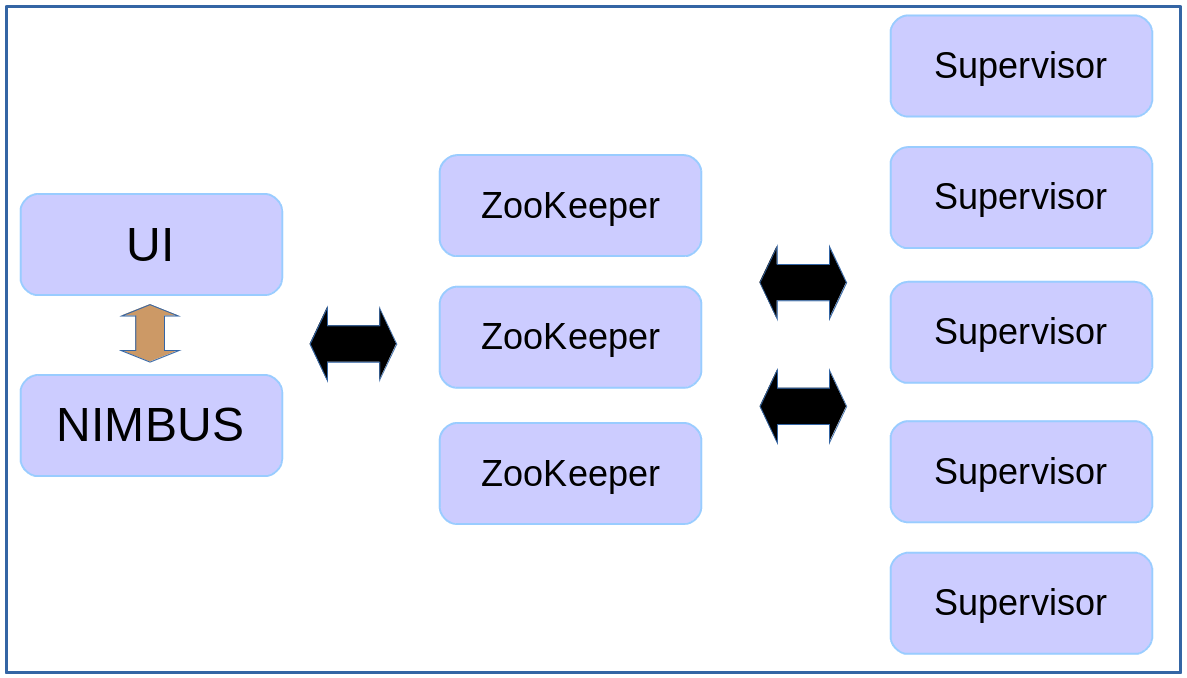
\includegraphics[width=0.5\textwidth,keepaspectratio=true]{figs/12/storm}
\begin{block}{System architecture}
\begin{itemize}

\item \textbf{Nimbus:} Like JobTacker in hadoop
\item \textbf{Supervisor:} Manage workers 
\item \textbf{Zookeeper:} Store meta data 
\item \textbf{UI:} Web-UI 
\end{itemize}
\end{block}
\end{frame}

% 
% \begin{frame}
% \frametitle{
% 
\includegraphics[width=0.25\textwidth,keepaspectratio=true]{figs/12/strat-logo}
% }
% \begin{itemize}
% \item Treats the underlying computation model as Direct Acyclic Graph
% \item Rich parallel programming model
% \item Introduces more Semantic information
% \item Allows to define own "operators" (think map, reduce)
% \item Analyzes and Compiles before execution
% \end{itemize}
% \end{frame}
% 
% \begin{frame} \frametitle{Architecture Comparison}
% \begin{center}
% 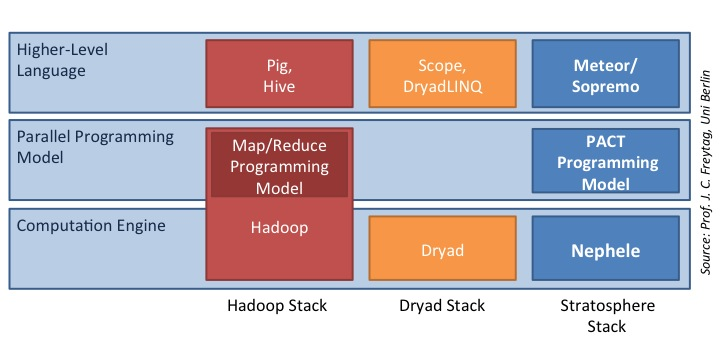
\includegraphics[width=\textwidth,keepaspectratio=true]{figs/12/SlidesFreytag/Slide01}
% \end{center}
% \end{frame}
% 
% \begin{frame} \frametitle{Focus Stratusphere Architecture}
% \begin{center}
% 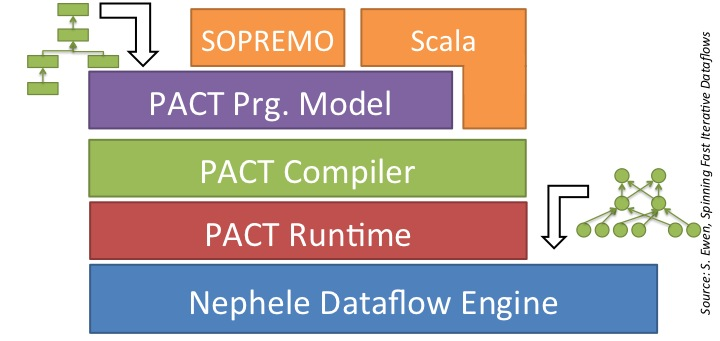
\includegraphics[width=\textwidth,keepaspectratio=true]{figs/12/SlidesFreytag/Slide06}
% \end{center}
% \end{frame}
% 
% \subsubsection{Pact Programming Model}
% %\begin{frame} \frametitle{Pact Programming Model}
% %\begin{center}
% %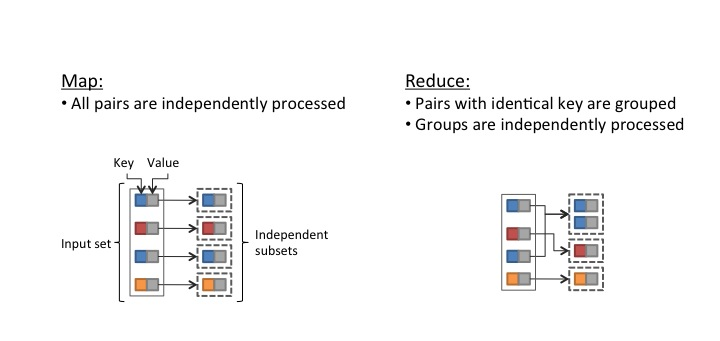
\includegraphics[width=\textwidth,keepaspectratio=true]{figs/12/SlidesFreytag/Slide07}
% %\end{center}
% %\end{frame}
% 
% \begin{frame} \frametitle{Extensions to MapReduce}
% \begin{center}
% \vspace{-2em}
% 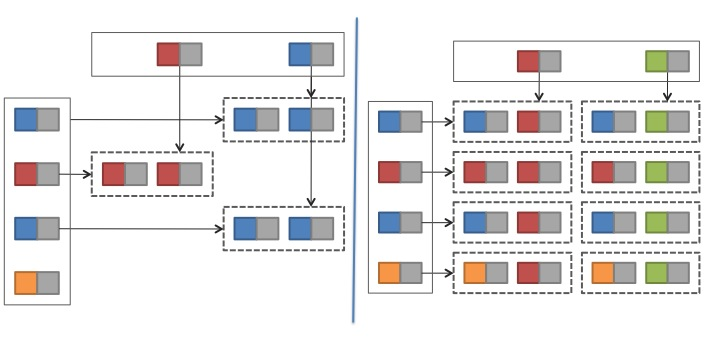
\includegraphics[width=.9\textwidth,keepaspectratio=true]{figs/12/SlidesFreytag/Slide12}
% \end{center}
% \begin{columns}
%  \column{0.49\textwidth}
%  Cross
% \begin{itemize}
% \footnotesize
% \item Cartesian Product
% \item Independent Processing of Elements
% \end{itemize}
%  \column{0.49\textwidth}
%  Match
% \begin{itemize}
% \footnotesize
% \item Equi-Join
% \item Independent Processing of Elements (CoGroup processes all at once)
% \end{itemize}
% \end{columns}
% 
% \end{frame}
% 
% \begin{frame} \frametitle{Pact (ProgrAmming ConTracts) Programming Model}
% \begin{center}
% 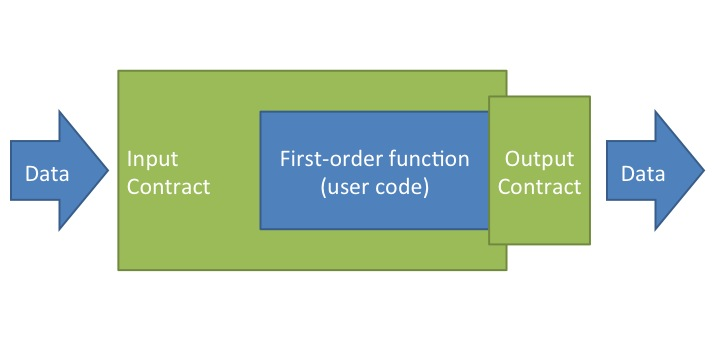
\includegraphics[trim=0px 80px 0px 120px,width=.7\textwidth,keepaspectratio=true]{figs/12/SlidesFreytag/Slide05}
% \end{center}
% \begin{columns}
%  \column{0.49\textwidth}
% Input Contract: 
% \begin{itemize}
% \item The Interface for your User function
% \item Generalized from map(key, value) and reduce(key, list(value))
% \end{itemize}
%  \column{0.49\textwidth}
% Output Contract: 
% \begin{itemize}
% \item Describes your produces output
% \begin{itemize}
% \item Sorted
% \item Unique key values
% \end{itemize}
% \end{itemize}
% \vspace{1.5em}
% \end{columns}
% \end{frame}
% 
% \subsubsection{Pact Compiler + Runtime}
% \begin{frame} \frametitle{Pact Compiler + Runtime}
% \begin{block}{Compiler}
% \begin{itemize}
% \item Memory Management
% \item Resolve Data Characteristics (Sorted, Unique)
% \end{itemize}
% \end{block}
% \pause
% \begin{block}{Runtime}
% \begin{itemize}
% \item Runtime observation of running program
% \item Performance Measurement, reordering
% \end{itemize}
% \end{block}
% \end{frame}
% 
% \begin{frame} \frametitle{Execution Engine: Nephele}
% \begin{center}
% 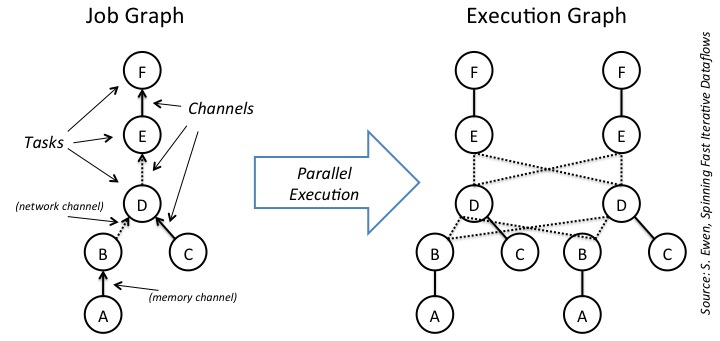
\includegraphics[width=\textwidth,keepaspectratio=true]{figs/12/SlidesFreytag/Slide02}
% \end{center}
% \end{frame}


\begin{comment}
\subsection{Dryad}

\subsubsection{Programming model}
\begin{frame}
 \frametitle{Main idea}
\begin{itemize}
 \item Developed by Microsoft
 \item In Map-Reduce all Maps must be completed before the Reduce
 \item Dryad generalize the concept
 \item The computation is modelled as a Direct Acyclic Graph
\end{itemize}
\end{frame}

\begin{frame} \frametitle{Structure}
\begin{center}
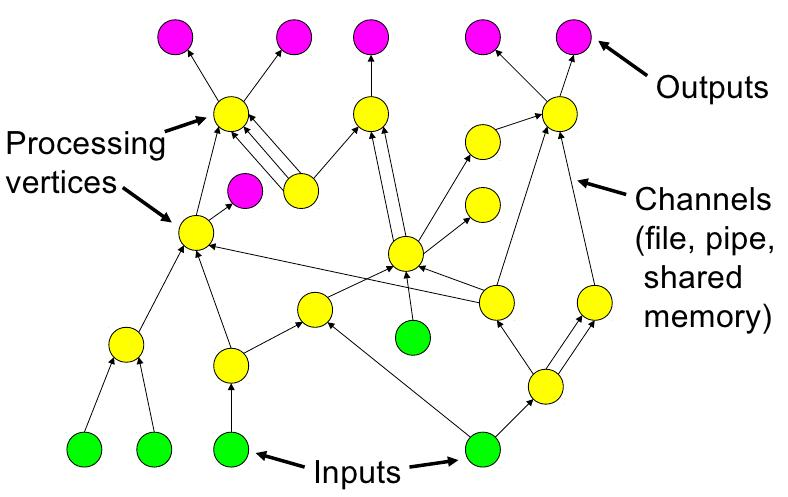
\includegraphics[width=\textwidth,keepaspectratio=true]{figs/12/dryad.jpg}
\end{center}
\end{frame}

\begin{frame}\frametitle{Example: Gravitational lens effect}
 \begin{block}{Input}
\begin{itemize}
 \item Table U: (starId, color)
 \item Table N: (starId, neighbourId)
\end{itemize}
 \end{block}

\begin{block}{Problem}
 Finding the pair of stars with similar colors.
\end{block}

\end{frame}
\begin{frame} \frametitle{Example: Gravitational lens effect}
\begin{columns}
 \column{0.45\textwidth}
\begin{itemize}
 \item X: join on starId
 \item D: distribute the data according to neighbourId
 \item M: merge inputs
 \item S: sort according to neighbourId
 \item Y: join neighbourId with starId of U
 \item H: filter distinct pairs
\end{itemize}

\column{0.1\textwidth}
\column{0.45\textwidth}
\begin{center}
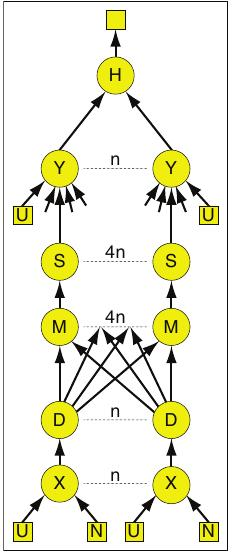
\includegraphics[scale=0.5,keepaspectratio=true]{figs/12/dryadquery.jpeg}
\end{center}
\end{columns}
\end{frame}

\begin{frame}
 \frametitle{Implementation}
\begin{itemize}
 \item Nodes are described as classes in C++
 \item The graph must be manually described in the code.
 \item The properties of the channels can be specified in the graph creation program
\end{itemize}
\end{frame}


\subsubsection{Framework}
\begin{frame}\frametitle{Framework characteristics}
\begin{itemize}
 \item Vertices are spawned across the network
 \item If a vertex fail, it can be restarted at another node
 \item There may be different copies of the same vertex running at the same time
 \item Messages across channels are buffered 
 \item Graph can be changed at runtime to optimize performance
\end{itemize} 
\end{frame}

\subsubsection{Dryad-Linq}
\begin{frame} \frametitle{Dryad-Linq}
\begin{itemize}
 \item Dryad is a low-level framework
 \item We need extensions to simplify usage
 \item Dryad-Linq is specialized on queries
\end{itemize}

\begin{block}{Linq}
 Part of the .NET framework. Adds support to queries
in all .NET languages
\end{block} 
\end{frame}

\begin{frame}[fragile]
\frametitle{Linq example}

\begin{lstlisting}
int[] numbers = new int[7] { 0, 1, 2, 3, 4, 5, 6 };
var numQuery = from num in numbers
               where (num % 2) == 0
               select num;
foreach (int num in numQuery) {
    Console.Write(num);
} 
\end{lstlisting}
 
\end{frame}

\begin{frame}
 \frametitle{DryadLinq overview}
DryadLinq processes the Linq code and:
\begin{itemize}
 \item creates the vertex code
 \item generates the graph
 \item passes the graph and the vertices to Dryad
\end{itemize}
\end{frame}

\subsection{Orleans}
\subsubsection{Programming model}
\begin{frame}
 \frametitle{Orleans}
\begin{itemize}
 \item Developed at Microsoft
 \item Aimed at integration Cloud+Client
 \item Actor-based computing
\end{itemize}

\begin{itemize}
 \item The basic unit of computation is the \textbf{grain}
 \item Grains collaborate in a \textbf{transaction}
 \item Each concurrent transaction uses a separate \textbf{activation} of each grain
 \item When a transaction has finished, the state of each grain is updated.
\end{itemize}

\end{frame}

\begin{frame}
 \frametitle{Details}
 \begin{block}{Grains}
  \begin{itemize}
   \item The developer defines a Grain Interface
   \item Many grains are created and their state is saved in permanent storage
   \item Whenever a process (maybe on a client) starts a transaction:
      \begin{itemize}
	\item each grain in the transaction is instantiated in a activation
        \item each activation is private to the transaction
        \item when the transaction has terminated the state of each activation is written to storage
        \item if conflicting changes across different transaction, changes are reconciled automatically
      \end{itemize}
  \end{itemize}

 \end{block}

\end{frame}

\subsubsection{Snippets}

\begin{frame}[fragile]
 \frametitle{Example}

\begin{block}{Grain interface}
\begin{lstlisting}[language=Java]
public interface ISimpleGrain : IGrain {
  AsyncValue<int> A { get; }
  AsyncValue<int> B { get; }
  AsyncCompletion SetA(int a);
  AsyncCompletion SetB(int a);
  AsyncValue<int> GetA();
  AsyncValue<int> GetB();
  AsyncValue<int> GetAxB();
}
\end{lstlisting}
\end{block}
\end{frame}

\begin{frame}[fragile] 
\frametitle{Example}
\begin{block}{Promises}
\begin{lstlisting}[language=Java]
AsyncValue<int> intPromise = grain.GetA();
intPromise.ContinueWith((int a) => {
  Console.WriteLine("Result: " + a.ToString());
},(Exception exc) => {
  Console.WriteLine("Error: " + exc.Message);
}).Ignore();
\end{lstlisting}
\end{block}
\end{frame}

\begin{frame}[fragile] 
 

\frametitle{Example}
\begin{block}{Promises advanced}
\footnotesize{
\begin{lstlisting}[language=Java]
AsyncCompletion setA = grain.SetA(3);
AsyncCompletion setB = grain.SetB(4);
AsyncCompletion set=AsyncCompletion.Join(setA,setB);
AsyncValue<int> get= 
    set.ContinueWith( () => { return grain.GetAxB(); });

AsyncCompletion result = get.ContinueWith(
(int x) => { Console.WriteLine("Result: " + x.ToString()); },
(Exception e) => { Console.WriteLine("Error: " + e.Message)}
);

try {
    result.Wait();
} catch(Exception exc) {
    Console.WriteLine("Error: " + exc.Message);
}

 
\end{lstlisting}

}
\end{block}
\end{frame}
\end{comment}

\section{Graph Processing}
\subsection{Motivations}
\begin{frame}
 \frametitle{Motivations}
\begin{center}
 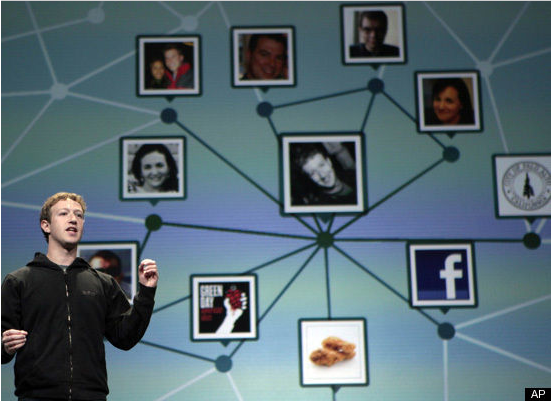
\includegraphics[keepaspectratio=true,width=0.45\textwidth]{figs/12/fb_opengraph}
\end{center}
\begin{block}{}
 Many big data sets are graphs:
\begin{itemize}
 \item World wide web graphs
 \item Social network topology
 \item Protein folding graphs
\end{itemize}
\end{block}
\end{frame}

\begin{frame}
\frametitle{Motivations}

 \begin{columns}
 \begin{column}{0.4\textwidth}
\begin{exampleblock}{Application domains}
\begin{itemize}
\item Computer networks,
\item Social networks,
\item Bioinformatics,
\item Chemoinformatics.
\end{itemize}
\end{exampleblock}

 \begin{block}{Graph representation}
%Graphs are now widely used for data modeling in several application domains for which identifying relationship patterns, rules, and anomalies is useful.
\begin{itemize}
\item Data modeling. % in several application domains,
\item Identifying relationship patterns and rules.
\end{itemize}

\end{block}
\end{column}
\begin{column}{0.6\textwidth}
\tiny{Protein structure} \includegraphics[scale=0.07]{figs/12/protein.eps}

\tiny{Chemical compound} 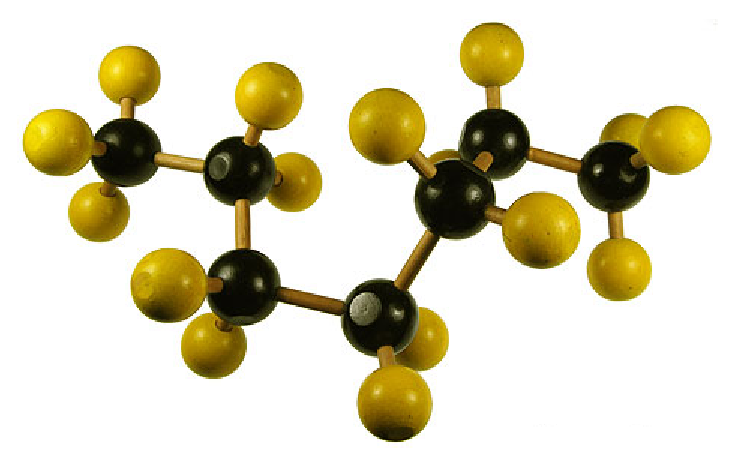
\includegraphics[scale=0.2]{figs/12/chemical.eps}

\tiny{Social network} \includegraphics[scale=0.04]{figs/12/socialnetwork.eps}
 \end{column}

\end{columns}
\end{frame}



\subsection{Pregel model}
\begin{frame}
 \frametitle{Pregel}

\begin{itemize}
 \item Developed at Google.
 %\item Based on the Bulk Synchronous Parallel model
 \item Algorithm based on a sequence of supersteps
 \item Each vertex in the graph is seen as a different process
 \item At each superstep, each vertex:
 \begin{itemize}
   \item Receives the list of messages sent to it during the last superstep
   \item Computes its new state
   \item Sends messages to other vertices
   \item Decides if it votes to halt
 \end{itemize}
 \item When all nodes vote to halt, the algorithm stops.
\end{itemize}
\end{frame}
% 
% \begin{frame}
%  \frametitle{BSP}
% \begin{center}
%  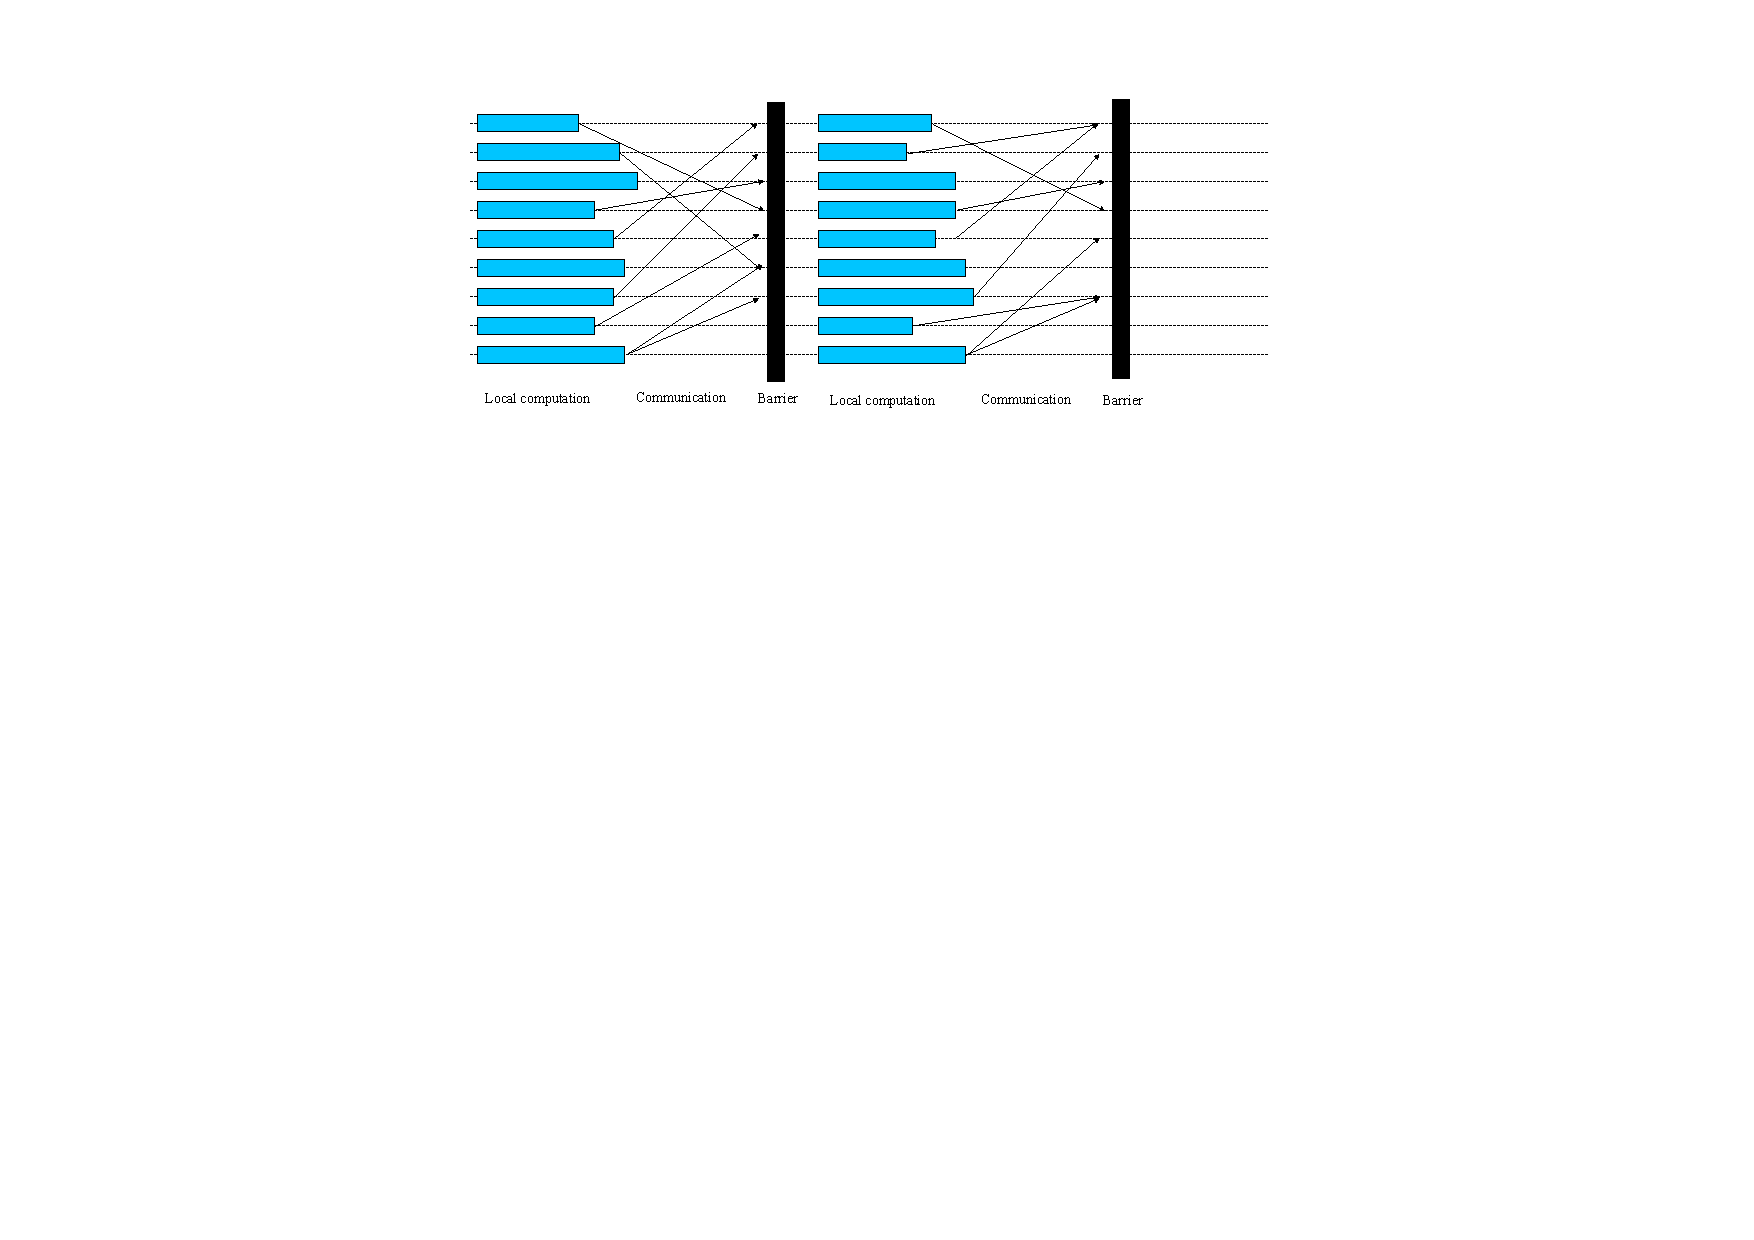
\includegraphics[keepaspectratio=true,width=\textwidth]{figs/12/bsp}
% \end{center}
% \end{frame}

\begin{frame}
 \frametitle{Framework}  
 \begin{itemize}
  \item Each process take control of a part of the graph 
  \item The vertices are divided between the nodes
  \item The order of computation inside each superstep is not important
  \item Can be built over MapReduce or other frameworks
 \end{itemize}
\end{frame}

\subsubsection{Sample Algorithms: SSSP}
\begin{frame}
 \frametitle{SSSP}
\begin{block}{Single source shortest path}
 Given a graph and a source vertex $s$, compute the distance from $s$ to all other vertices.
\end{block}

\begin{block}{Centralized solution}
 Run a breadth-first search.
\end{block}
\end{frame}

\begin{comment}
\begin{frame}{SSSP with MapReduce}

\begin{figure}
	\begin{overprint}
\onslide<1|handout:1>\centering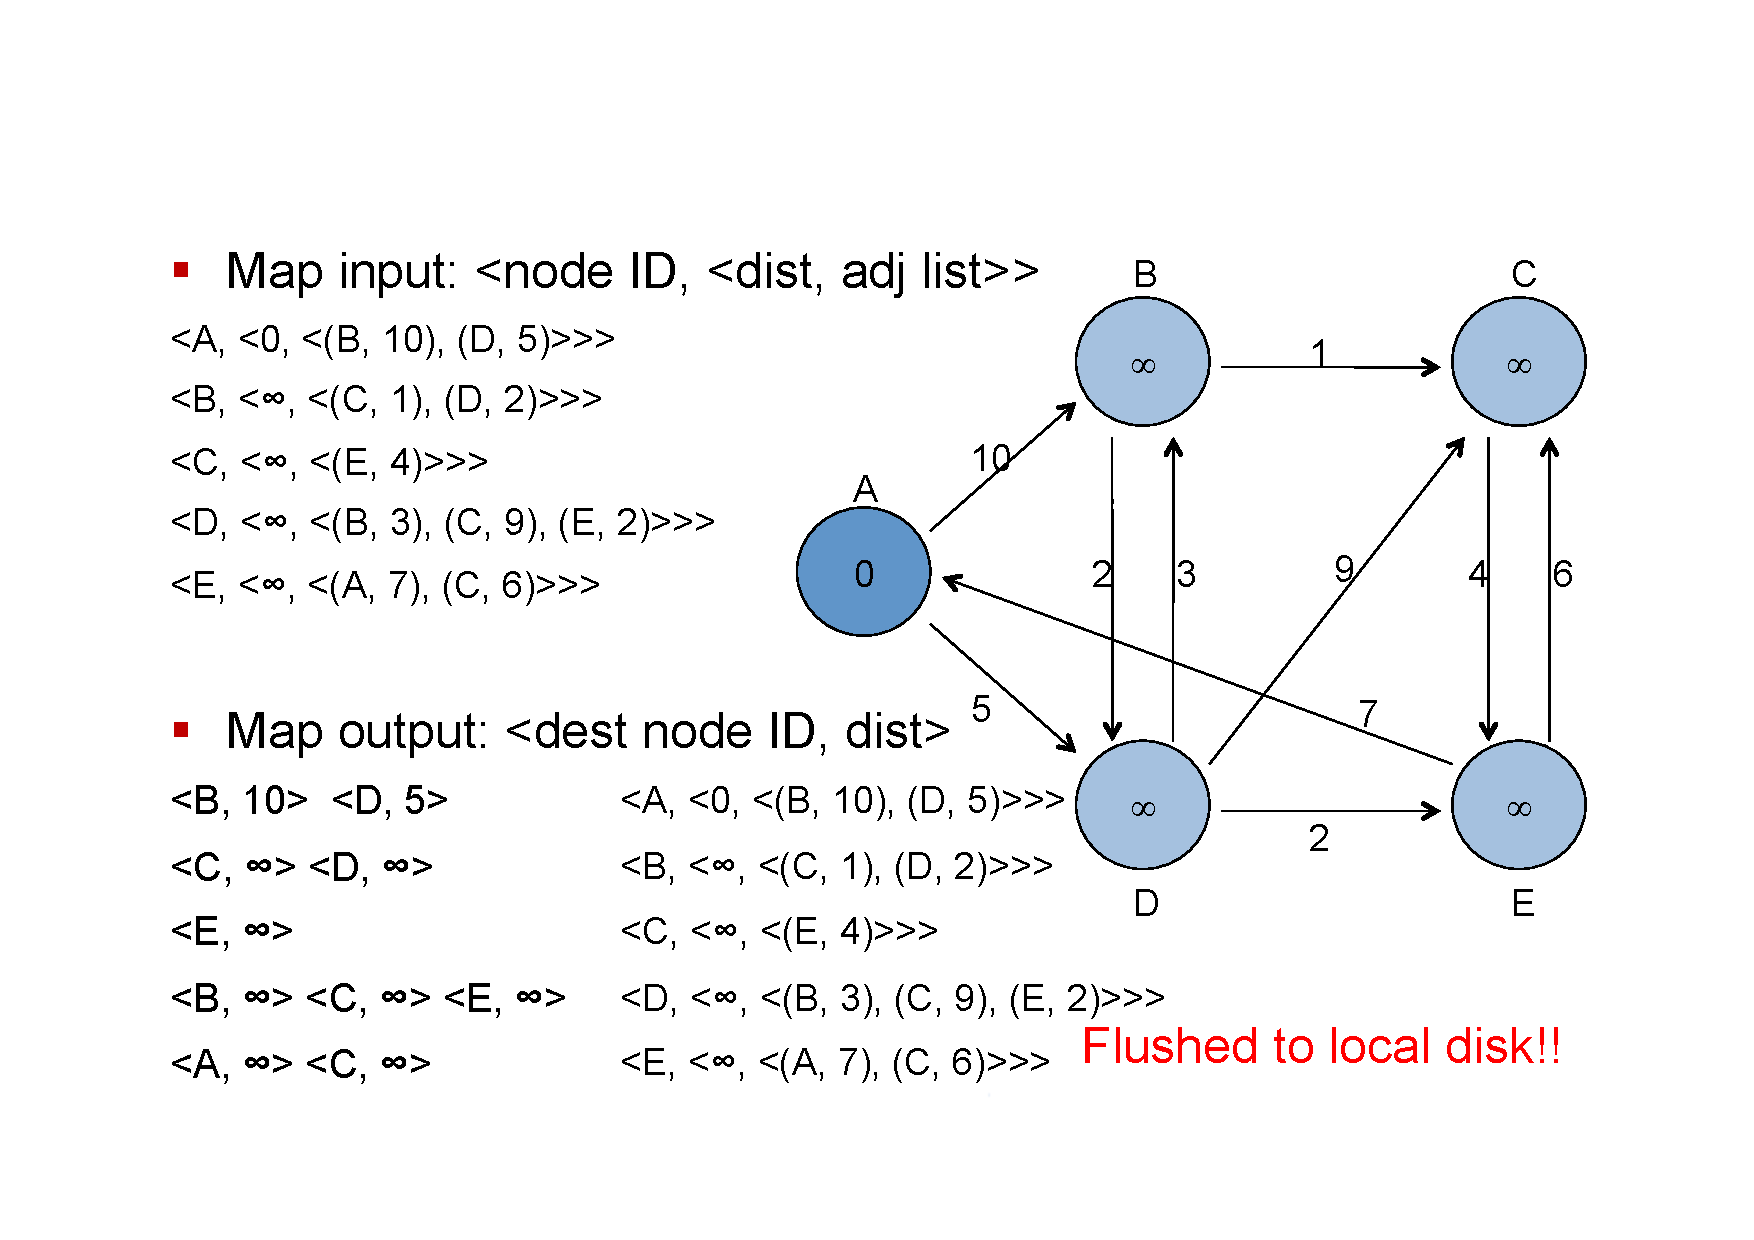
\includegraphics[width=10cm,page=1]{figs/12/sssp.pdf}
\onslide<2|handout:2>\centering\includegraphics[width=10cm,page=2]{figs/12/sssp.pdf}
\onslide<3|handout:3>\centering\includegraphics[width=10cm,page=3]{figs/12/sssp.pdf}
\onslide<4|handout:4>\centering\includegraphics[width=10cm,page=4]{figs/12/sssp.pdf}
\end{overprint}
\end{figure}
\end{frame}

\end{comment}

\begin{frame}[fragile]
 \frametitle{Pregel solution}
\begin{algorithm}[H]
$\INTEGER\ \textit{dist} \gets (\mathbf{this} = \textit{source})\ ?\ 0\ :\ +\infty$\;
\BlankLine
\PROCEDURE{$\textsf{compute}(\textit{messages})$}{
  $\INTEGER\ \textit{newdist} \gets \textsf{min}(\textit{messages})$\;
  \eIf{$\textit{newdist} < \textit{dist}$}{
    $\textit{dist} \gets \textit{newdist}$\;
    \For{$\textsc{Edge}\ e \in \mathbf{this}.\textsf{getNeighbors}()$}{
       $\textsf{sendMessage}(e,\textit{dist}+e.\textit{value}())$;
    }
  }{
    $\textsf{voteToHalt}()$\;
  }
}
\caption{SSSPVertex}
\end{algorithm}
\end{frame}


\begin{frame}{Shortest path}
\begin{figure}
\begin{overprint}
\onslide<1|handout:1>\centering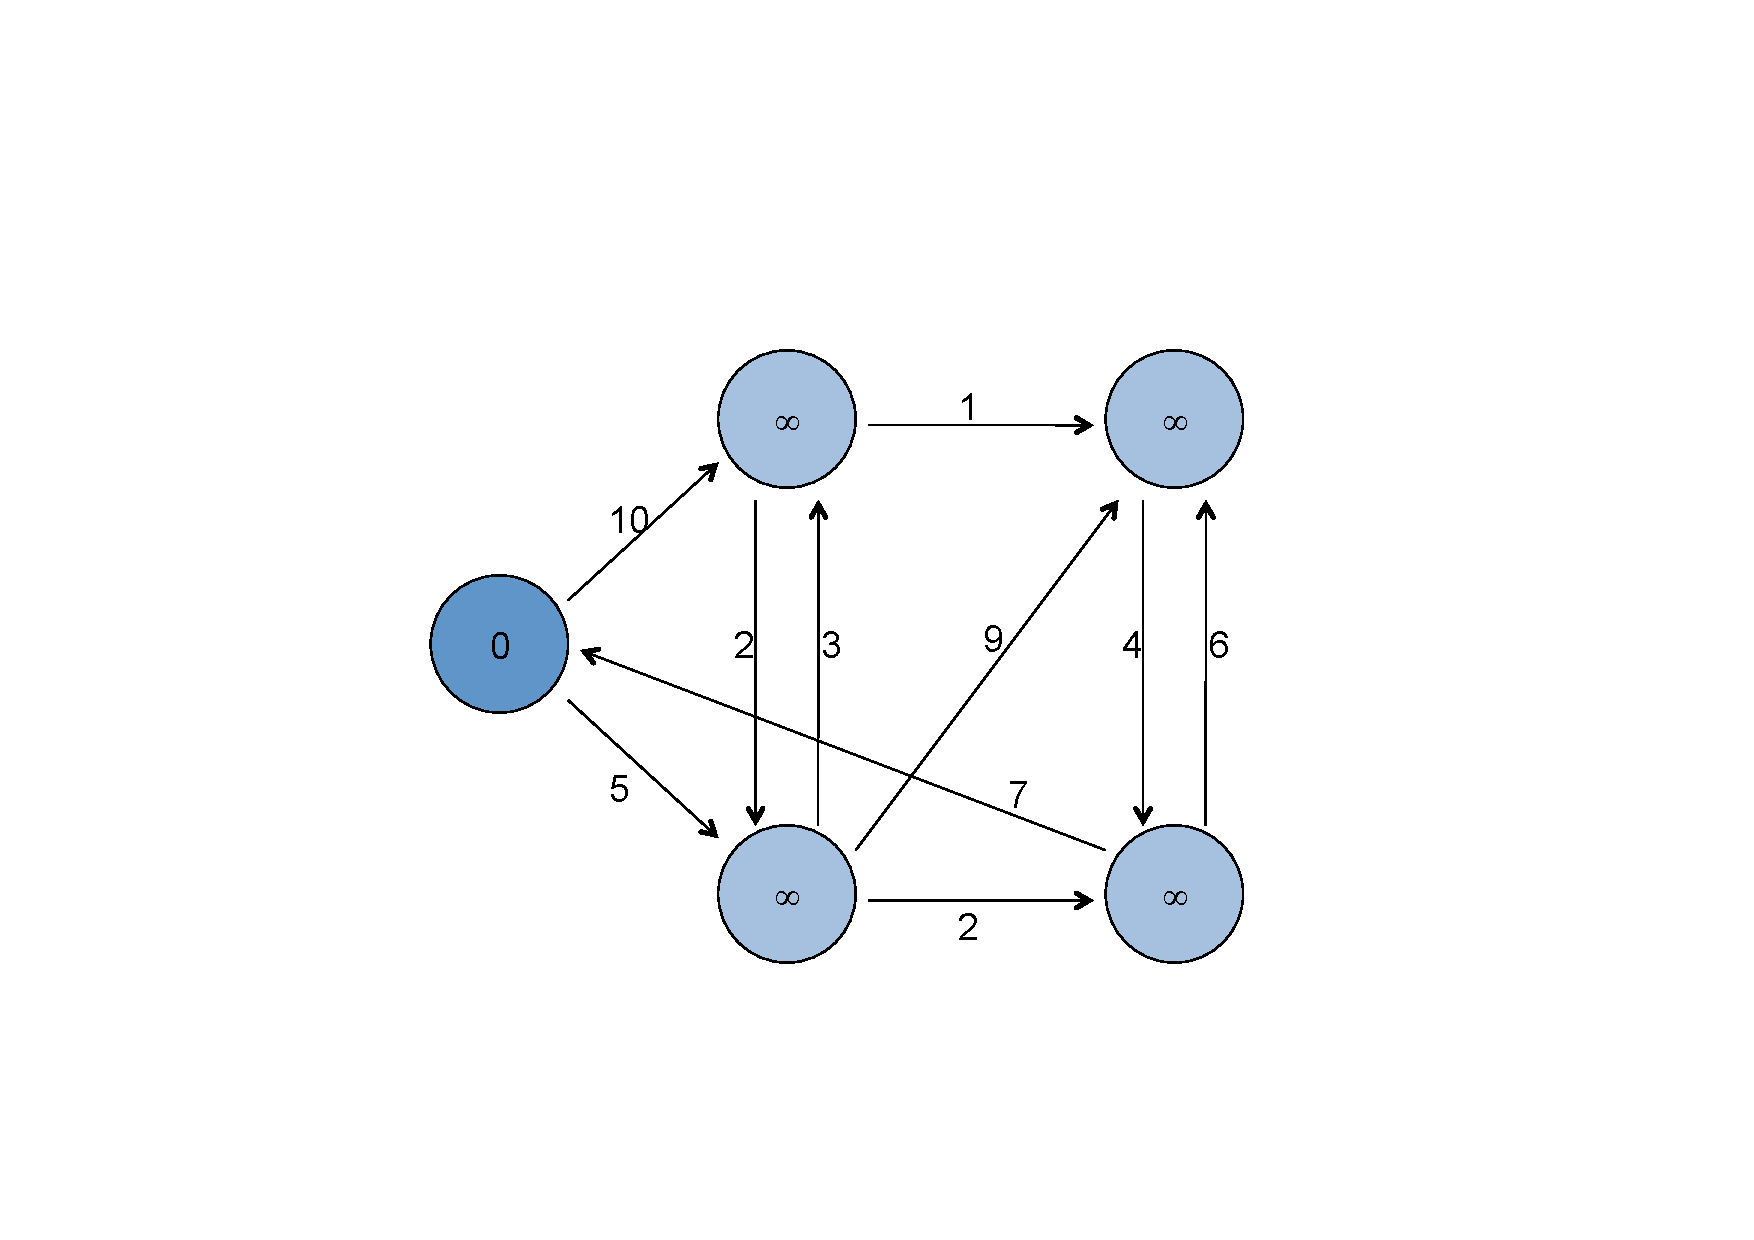
\includegraphics[width=8cm,page=1]{figs/12/shortest.pdf}
\onslide<2|handout:2>\centering\includegraphics[width=8cm,page=2]{figs/12/shortest.pdf}
\onslide<3|handout:3>\centering\includegraphics[width=8cm,page=3]{figs/12/shortest.pdf}
\onslide<4|handout:4>\centering\includegraphics[width=8cm,page=4]{figs/12/shortest.pdf}
\onslide<5|handout:5>\centering\includegraphics[width=8cm,page=5]{figs/12/shortest.pdf}
\onslide<6|handout:6>\centering\includegraphics[width=8cm,page=6]{figs/12/shortest.pdf}
\onslide<7|handout:7>\centering\includegraphics[width=8cm,page=7]{figs/12/shortest.pdf}
\onslide<8|handout:8>\centering\includegraphics[width=8cm,page=8]{figs/12/shortest.pdf}
\onslide<9|handout:9>\centering\includegraphics[width=8cm,page=9]{figs/12/shortest.pdf}
\end{overprint}
\end{figure}
	
\end{frame}	



\subsubsection{Available implementations}
\begin{frame}[fragile]
 \frametitle{Available implementation}
Both based on Apache Hadoop
\begin{block}{GoldenOrb}
\begin{itemize}
 \item Developed by an independent company, sponsored by Ravel (Austin TX)
 \item Launched June 2011
\end{itemize}
\end{block}

\begin{block}{Apache Giraph}
 \begin{itemize}
 \item Developed in Apache Incubator
\end{itemize}
\end{block}

\begin{lstlisting}[language=Java,basicstyle=\tiny]

public class MyVertex extends Vertex<IntWritable, IntWritable, IntMessage>{
 ...
 public void compute(Collection<IntMessage> messages) {
    ...
    sendMessage(new IntMessage(dest, new IntWritable(42)));
 }
}
\end{lstlisting}

\end{frame}

\subsection{Blogel}
\begin{frame}
 \frametitle{Blogel}

\begin{itemize}

 \item A block-centric framework for distributed computation  on large graphs.
 \item From \textbf{'Think Like a Vertex'} to \textbf{'Think Like a Block'} 
 \item A block refers to a connected subgraph of the graph.
 \item Message exchanges occur among blocks.
 
\end{itemize}
\end{frame}

\begin{frame}
 \frametitle{Blogel}
\begin{center}
 \includegraphics[keepaspectratio=true,width=0.5\textwidth]{figs/12/blogel}
\end{center}
\begin{block}{}
Three types of jobs:
\begin{enumerate}
 \item Vertex-centric graph computing, where a worker is called a V-worker. 
 \item Graph partitioning which groups vertices into blocks, where a worker is called a partitioner. 
 \item Block-centric graph computing, where a worker is called a B-worker. 
\end{enumerate}
\end{block}
\end{frame}


\begin{frame}
 \frametitle{Blogel}

\begin{itemize}
 \item Blogel operates in three computing modes, depending on the application.
 \begin{itemize}
   \item \textbf{B-mode:} Only block-level message exchanges are allowed. A job terminates when all blocks voted to halt and there is no pending message for the next superstep. 
   \item \textbf{V-mode:} Only vertex-level message exchanges are allowed. A job terminates when all vertices voted to halt and there is no pending message for the next superstep. 
   \item \textbf{VB-mode:} vertex-level message exchanges and block-level message exchanges are allowed. 
 \end{itemize}
\end{itemize}
\end{frame}

\section{Q and A}
\begin{frame}
 \frametitle{That's it. Why was this important?}
%  \pause
 \begin{center}
%  \only<2>{\url{https://github.com/rtreffer/hadoop-cablegate}}
%  \only<3>{ 
 
 \includegraphics[keepaspectratio=true,scale=0.45]{figs/12/questions}

\footnotesize Questions?\\
sabeur.aridhi@unitn.it
 \end{center}
\end{frame}

\end{document}
